% arara: xelatex
% arara: xelatex
% arara: xelatex


% options:
% thesis=B bachelor's thesis
% thesis=M master's thesis
% czech thesis in Czech language
% english thesis in English language
% hidelinks remove colour boxes around hyperlinks

\documentclass[thesis=B,english]{FITthesis}[2019/12/23]

%\usepackage[utf8]{inputenc} % LaTeX source encoded as UTF-8
% \usepackage[latin2]{inputenc} % LaTeX source encoded as ISO-8859-2
% \usepackage[cp1250]{inputenc} % LaTeX source encoded as Windows-1250

% \usepackage{subfig} %subfigures
\usepackage{amsmath} %advanced maths
\usepackage{booktabs}
% \usepackage{amssymb} %additional math symbols

%\usepackage[demo]{graphicx}
\usepackage{subcaption}

\usepackage{dirtree} %directory tree visualisation
\usepackage[colorinlistoftodos]{todonotes}
\usepackage{nicematrix}

% % list of acronyms
% \usepackage[acronym,nonumberlist,toc,numberedsection=autolabel]{glossaries}
% \iflanguage{czech}{\renewcommand*{\acronymname}{Seznam pou{\v z}it{\' y}ch zkratek}}{}
% \makeglossaries

% % % % % % % % % % % % % % % % % % % % % % % % % % % % % % 
% EDIT THIS
% % % % % % % % % % % % % % % % % % % % % % % % % % % % % % 

\department{Department of Applied Mathematics}
\title{Detection of Organs in CT Images Using Neural Networks}
\authorGN{Ivana} %author's given name/names
\authorFN{Hacajová} %author's surname
\author{Ivana Hacajová} %author's name without academic degrees
\authorWithDegrees{Ivana Hacajová} %author's name with academic degrees
\supervisor{Ing. Jakub Žitný}
\acknowledgements{First, I would like to thank Ing. Jakub Žitný for supervising my thesis, who was very enthusiastic about my project and always eager to help, providing me with useful resources. I am also very grateful for the support from my family and close friends, especially during the strange times of the COVID-19 pandemic, which left many people in uncertain and difficult situations. I am also very thankful to the organisers of VerSe`19: Large Scale Vertebrae Segmentation Challenge for providing us with very valuable CT data.}

\abstractEN{This thesis contains research of the field of medical imaging, classical methods of image segmentation, computed tomography and convolutional neural networks. The practical part involves implementation of an architecture of 3D UNet for segmentation of the spine and specific vertebrae from CT scans. Furthermore, this architecture is compared to its 2D counterpart.}

\abstractCS{Táto práca sa zaoberá výskumom zobrazovacích metód v medicíne, klasických prístupov k segmentácii obrázkov, CT a konvolučným neuronovým sietiam. Praktickou časťou je implementácia architektúry 3D UNet pre segmentáciu chrbtice a jednotlivých stavcov z CT obrázkov a jej porovnanie s jej 2D verziou.}

\placeForDeclarationOfAuthenticity{Prague}
\keywordsCS{zobrazovacie metódy v medicíne, konvolučné neuronové siete, segmentácia, CT, chrbtica, stavce}

\keywordsEN{medical imaging, convolutional neural networks, segmentation, CT, spine, vertebrae}
\declarationOfAuthenticityOption{5} %select as appropriate, according to the desired license (integer 1-6)
\website{https://github.com/iVonka/Detection-of-Organs-in-CT-Images-Using-Neural-Networks} %optional thesis URL


\begin{document}

% \newacronym{CVUT}{{\v C}VUT}{{\v C}esk{\' e} vysok{\' e} u{\v c}en{\' i} technick{\' e} v Praze}
% \newacronym{FIT}{FIT}{Fakulta informa{\v c}n{\' i}ch technologi{\' i}}

\setsecnumdepth{part}
\chapter{Introduction}
%Aktuálnost tématu
The year is 2020. I can say with confidence, that the last decade belonged to AI. Modern hardware finally allowed for solving tasks deemed too computationally demanding before. Machine learning algorithms are already present in our daily activities, even if we do not know about them. They are responsible for solving numerous tasks: predictions, recommendations, object detection and recognition and many more.  

%Čím je téma prospěšné pro společnost a proč se problematikou zabýváme
I have always wanted to connect my field (computer science) with natural sciences. Medical industry offers various applications of machine learning, one of which is image analysis. Medical images have become an integral part of diagnosis and treatment of patients. It comes just natural to try to automize the process of their analysis and diagnosis. 

%Stanovenícíle(ů)práce
The focus of my thesis is detection of organs in CT images using modern approaches, such as neural nets. This covers researching the medical imaging field, state-of-the-art methods for image analysis and also implementing my own prototype for organs detection with the data set of my choice. 

%Představení struktury celé práce – obsah jednotlivých kapitol
In the first chapter of my thesis I will talk about how the field of medical imaging developed throughout the history, starting with X-Rays. I will focus on classical methods used for medical image processing, which proved to be efficient, but are being replaced by machine learning algorithms. The following chapter introduces CT as a technology and some important characteristics of the CT scans. The third chapter is a review of convolutional neural networks and their variations proposed for different scenarios and uses in image processing. And last, but not least, I will describe the work I have done implementing a neural networks model for detection of organs in CT images. My task is segmentation of a spine and specific vertebrae. 
\chapter{Aim of the Thesis}
\label{ch:aim}
The aim of this thesis is to research techniques used in the medical imaging domain and implement my own model for segmentation of organs using neural nets.

In the literature review I will look at the historical milestones that shaped the medical imaging domain. I will introduce techniques for image analysis in medicine popular in the past, as well as those used nowadays. Furthermore I will focus on CT images and the technology behind them. The approach of my choice is convolutional neural networks and their variations that have recently gained popularity. 

The practical part of my work will cover implementing my own prototype model for segmentation tasks over medical images. The data set I will work with consists of CT images of human spines. I will try to segment spine and also specific vertebrae from these images. I will compare my results with results of already existing models, discuss them. My prototype code has to be published and be reproducible. 

\setsecnumdepth{all}

%----LITERATURE REVIEW----%
\chapter{Medical Image Analysis}
\label{ch:medical-image-analysis}
In the first chapter of my thesis I am going to talk about Medical Image Analysis. I will briefly describe discoveries and milestones in medical imaging that led to the origin of the field. I will continue with introducing techniques and approaches used at its beginnings and are still relevant to this day. 

%----SECTIONS----%
\section{Medical Imaging}
Medical imaging is an integral part of the modern medicine. It refers to the techniques that produce visualisations of various parts of the human body. These images are usually used for diagnoses and treatment of patients. Its use became widespread in the 20th century, as many of the devices used for medical imaging were invented in the past hundred years.  

 It all started in 1895 with X-Rays. Wilhelm Conrad Röntgen was experimenting with a cathode-ray tube (vacuum tube with electron beams that strikes a phosphorescent screen) \cite{glasser1993}. He noticed the tube was emitting a fluorescent glow. This ray could pass through various substances and human tissues, except for bones and metal objects, casting shadows. One of his first experiments was an image of his wife's hand \ref{fig:first-rtg}. The news about X-Ray spread quickly and left the scientific community amazed. X-Ray started to be heavily used in medicine and physics very soon after its invention. However, unwanted side-effects were observed. X-Rays have a very short wavelength (1 angstrom). Therefore, they can penetrate materials visible light (6000 angstroms) cannot. This can cause serious damage to human bodies like skin burns or even loss of limbs from early exposures. 
 
\begin{figure}[ht]
    \centering
    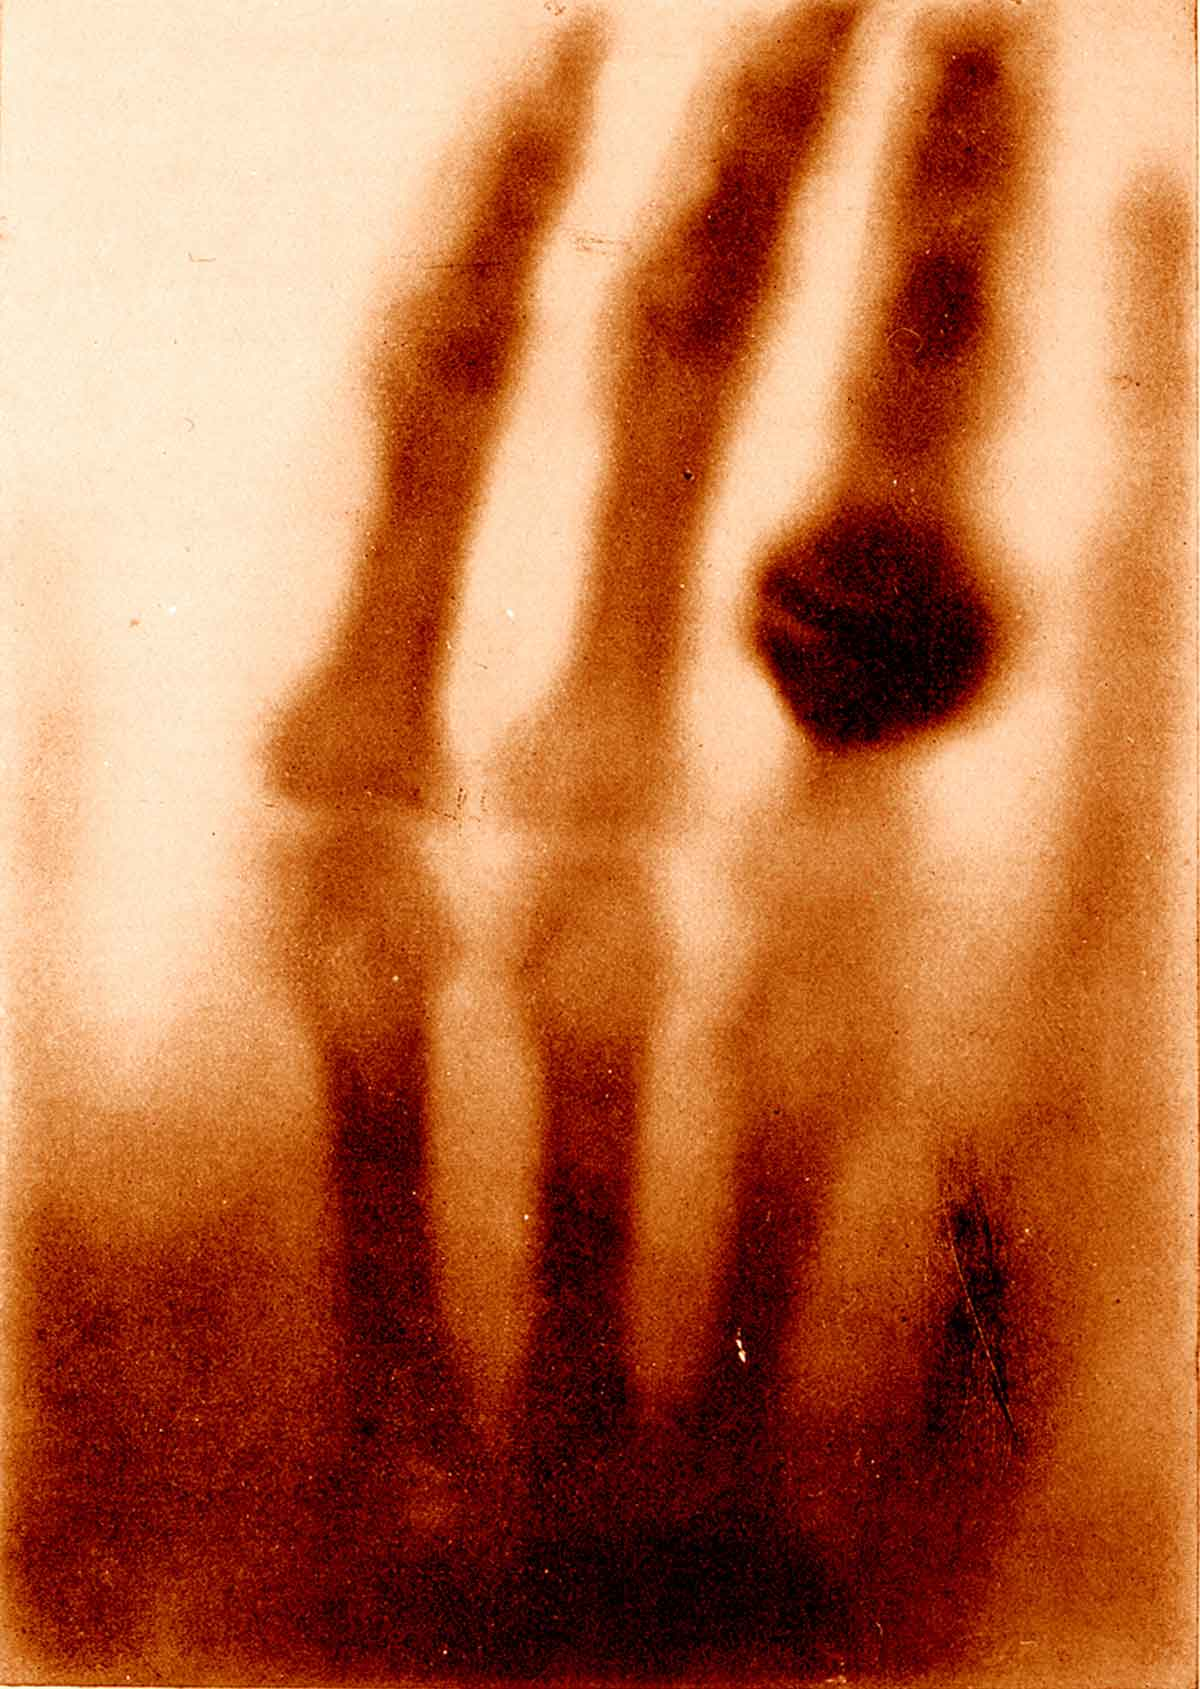
\includegraphics[width=150pt]{images/first-rtg.jpg}
    \caption[The hand of Mrs. Wilhelm Roentgen: the first X-ray image, 1895]{The hand of Mrs. Wilhelm Roentgen: the first X-ray image, 1895 \cite{glasser1993}}
    \label{fig:first-rtg}
\end{figure}

 Another important milestone in the medical field was ultrasound. Unlike X-Ray, ultrasound had been already used in other areas (localisation of submarines, detection of flaws in metals) before its introduction into medical diagnosis. Ultrasound is a high-frequency sound. So high, a human ear cannot detect it. A probe is used to transmit these waves into patient's body. The sound-waves echo from internal tissues and are reflected back to the probe. Then, an image representation is computed from the reflections. In 1958, Ian Donald and his team published the first paper about the use of ultrasound in obstetrics and gynaecology. They managed to get the first image of a fetus. Ultrasound gained popularity also due to its non-invasiveness and harmlessnes (in comparison to X-Rays). By 2000, modern real-time scanning machines with 3D/4D options were already available on the market.
 
 After 60 years from the invention of X-Rays, a biomedical engineer Godfrey Hounsfield came up with an idea to create three-dimensional scans of the human body. K. B. Bhattacharyya summarised Hounsfield's journey in his article \cite{bhattacharyya2016}: He wanted to develop a software that would compile X-Ray images from various angles into a 3D one. He succeeded and constructed the first CAT (computed axial tomography) scanner. In 1971, CAT scanners began to be used in hospitals. They could produce scans of brains, which was very helpful in diagnosing brain lesions. Hounsfield worked very hard to improve his inventions, so other parts of the body could be imaged as well. He was awarded a Nobel Prize for Medicine in 1979. I will talk more about C(A)T scans in the later chapters.
 
In 1973 we could witness another breakthrough in the medical imaging domain - MRI (magnetic resonance imaging). First, we need to go back to its roots in the 1930s. Austrian scientist Isidor Isaac Rabi discovered, that molecules passing through a magnetic field emit specific radio waves and change their spins. Each atom or molecule resonates with different frequencies that can be used to identify them and distinguish between types. This phenomenon is known as nuclear magnetic resonance (NMR). Paul Lauterbur found a way for NMR to produce images. He used the signals from different atoms to build the pictures \cite{lauterbur1973}. In contrast to X-Rays or CT, MRI does not emit radiation and is generally safer. MRI works well with soft tissues, for example brain.

Nowadays, all these imaging techniques (and others) are widely used and are a crucial part of the process of diagnosis and treatment. All the devices have been keeping up with the latest technology and are able to produce better results leading to more accurate diagnosis. Additionally, potential health risks from their use have been more thoroughly researched and reduced.

According to data from Eurostat \cite{eurostat2019}, the number of examinations by medical imaging techniques is still on a rise worldwide, as the technology is becoming more available. In Slovakia, there were 42,468 examinations performed using MRI in 1996. 20 years later it was 333,599. Similarly, the number of CT scans has grown 6-times in the same time period. Naturally, there was a need for image processing techniques that would either enhance some features of these images, make them more easily interpretable for doctors or even detect specific objects. Furthermore, we wanted to automatise these processes. 




 



\section{Classic methods}
The field of Medical Image Analysis originated from Computer Vision in the early 1990s. Researchers with CV background started applying already established mathematical methods to medical images. In 1996 this newly emerging field got its own archival journal \textit{Medical Image Analysis}. To this day, it is a leading medium that publishes new research results from this area \cite{wells2016}.

In this section I would like to focus on fundamental approaches for image segmentation used at the beginnings. Segmentation is a process of separating objects from the background or from other objects. We can do this by identifying every pixel that belongs to this object or finding its boundaries. In the medical field, segmentation can be used for automated classification of blood cells, detection of tumors, measuring tumor volume and its response to therapy and many more.

\subsection{Thresholding}
Thresholding \cite{thresholding} is a technique based on finding a grey level -- threshold \textit{T}. Every pixel value is compared to this threshold and then assigned to either object or background. Suppose we have an image or its part \textit{f(x,y)}. The thresholded image \textit{g(x,y)} is defined as:

\begin{equation}
    g(x,y) = 
    \left\{\begin{matrix}
    1  &  if (x,y) > T \\ 
    0  &  if (x,y) \leq T
    \end{matrix}\right.
\end{equation}

If the histogram of our image is bimodal (a histogram with two separated peaks), we can assume its peaks represent an object and a background. In this case, we can use one threshold for the whole image. This is called \textit{global} thresholding. 

The global threshold can be chosen manually -- by looking at the histogram and choosing the grey level value at the bottom of the valley separating the peaks. There are also methods to automatise this process. Otzu's method finds the threshold that minimizes intra-class variance, which he shows is the same as maximizing inter-class variance \cite{otzu1979}.  

\textit{Global} thresholding does not always provide sufficient results. If the object has various intensity values, isn't on a contrasting background or is noisy, a different method has to be used. One of the solutions is \textit{local (adaptive)} thresholding. The image is divided into overlapping rectangular regions. A histogram is computed for each of these subimages and then the threshold for this region is chosen. This method is computationally more demanding than finding a \textit{global} threshold. 

Medical images are often blurry, noisy, with low contrast. Histrograms of such images are not bimodal, which causes problems with finding the right threshold. Some pre-processing techniques can help in such situations. We can try to smooth out the edges using various filters. Filters usually have a NxN shape, where N = 3, 5, 7, etc. 

One of the filters is \textit{mean} filter. For every pixel in the picture we find the average of the pixels in its local neighbourhood and that is its new value. Another common filter is \textit{median} filter, which computes the median value for for the neighbouring region. These filters change the histogram in a way that makes it possible to select the threshold. 

\subsection{Region Growing}
The region growing method \cite{medical-imaging-handbook}, as opposed to thresholding, is based on finding connected regions of pixels with similar values. The first step of the algorithm is to select one or more seeds -- pixels that belong to the object. 

The next step is checking all neighbouring pixels, whether they are similar enough to be added to the growing region. The similarity criterion is called uniformity test. This algorithm continues until there are no more pixels that can be added to the region. All the pixels that have been added to the region represent the object. 

The choice of the uniformity test is crucial, the result of region growing is heavily dependant on it. One of the tests can be to compare a pixel value to the mean of the already found region. A threshold for accepting pixels needs to be set. If the difference between the value and the mean is smaller than the threshold, the pixel is added to the region.

Region growing is a very simple technique. It can segment objects with predefined properties. It is computationally not demanding, as it visits every pixel a limited amount of times. On the other hand, it is very sensitive to noise.


\subsection{Watershed Algorithm}
Another region-based method is watershed algorithm \cite{medical-imaging-handbook}. This process can be viewed as filling valleys with water. 

First, seeds for the algorithm need to be chosen. Every object in the image, including the background, needs to be marked by a seed. These can be chosen by an expert or by some automated algorithm specific for the given domain.

We can look at the image as if it were a topographic map. Dark pixels represent valleys, bright ones represent mountaintops. The seeds represent holes in the valleys. Through these holes, water is flowing into their respecting valleys. At one point, waters from two different `lakes' meet. This is where we build a dam -- a border between two objects in the picture.

\subsection{Edge-based Segmentation Techniques}
Locating edges of objects is another way to segment images \cite{medical-imaging-handbook}. Edges in a picture \textit{f(x,y)} are defined by the local intensity gradient. Gradients approximate the first-order derivative of the image-function. The magnitude of a gradient can be calculated as

\begin{equation}
\label{eq:magnitude}
    \left | G \right | = \sqrt{ \left [ {G_{x}}^{2} + {G_{y}}^{2} \right ] } = \sqrt{\left [ \left ( \frac{\partial f}{\partial x}  \right )^{2} \right ] + 
\left [ \left ( \frac{\partial f}{\partial y}  \right )^{2} \right ]
}
\end{equation}

where \textit{$G_{x}$} is a gradient in the \textit{x} direction and \textit{$G_y$} is a gradient in the \textit{y} direction. We can look at them as gradients in the horizontal and vertical directions. Magnitude can be displayed as an image, where it is proportionally represented by grey level values. 

There are a lot of popular gradient operators to compute approximations of derivatives. They are usually filters that use convolution. Convolution is an operation, that computes weighted summations of values in local neighbourhoods. 

The filters have usually two kernels, so both horizontal and vertical changes can be detected. These gradients are then combined using \ref{eq:magnitude} creating the gradient magnitude image. Some of the filters are:

\textit{Sobel edge operator}
\[ 
\begin{array}{cc}

    \begin{bmatrix}
    -1 & -2 & -1 \\
    0 & 0 & 0 \\
    1 & 2 & 1 
    \end{bmatrix} 
                    
    \begin{bmatrix}
    -1 & 0 & 1 \\
    -2 & 0 & 2 \\
    -1 & 0 & 1
    \end{bmatrix}
    
\end{array}
\]
\pagebreak

\textit{Prewitt operator}

\[ 
\begin{array}{cc}

    \begin{bmatrix}
    1 & 1 & 1 \\
    0 & 0 & 0 \\
    -1 & -1 & -1 
    \end{bmatrix} 

    \begin{bmatrix}
    1 & 0 & -1 \\
    1 & 0 & -1 \\
    1 & 0 & -1
    \end{bmatrix}
    
\end{array}
\]

\textit{Roberts Cross operator}
\[ 
\begin{array}{cc}

    \begin{bmatrix}
    1 & 0 \\
    0 & -1 
    \end{bmatrix} 

    \begin{bmatrix}
    0 & 1 \\
    -1 & 0 
    \end{bmatrix}
    
\end{array}
\]

Gradient operators are often followed by a thresholding operation. In this step it is decided, whether an edge has been found or not. The result of this operation is a binary image containing the detected edges.  

Apart from the first-order derivatives, also the second-order derivatives can be used to detect boundaries of objects. Peaks in the first-order correspond to zeros in the second-order derivatives. \textit{Laplacian operator} is able to approximate them. The operator $\nabla^2$ of an image function \textit{f(x,y)} is defined as:

\begin{equation}
    \nabla^2f(x,y) = \frac{\partial^2 f(x,y)}{\partial x^2} + 
    \frac{\partial^2 f(x,y)}{\partial y^2}
\end{equation}

Convolutional masks that approximate \textit{Laplacian operator} can be:

\[ 
\begin{array}{cc}

    \begin{bmatrix}
    0 & -1 & 0 \\
    -1 & 4 & -1 \\
    0 & -1 & 0 
    \end{bmatrix} 

    \begin{bmatrix}
    -1 & -1 & -1 \\
    -1 & 8 & -1 \\
    -1 & -1 & -1
    \end{bmatrix}
    
    \begin{bmatrix}
    1 & -2 & 1 \\
    -2 & 4 & -2 \\
    1 & -2 & 1
    \end{bmatrix}
    
\end{array}
\]

After applying \textit{Laplacian operator}, edges need to be located. Those are pixels where \textit{Laplacian} passes through zero (pixels, where the operator changes signs). This occurs when the pixel intensity changes rapidly.

\subsection{K-Means Clustering}
Clustering in general is a term which describes a problem of finding groups among a set of objects. These groups are called clusters. Clustering works with unlabeled objects and the goal is to find some categories data is organised into.

There are many ways for describing a cluster \cite{clustering}: The easiest way to understand what a cluster is, is to look at it as a group of objects, where all the objects are similar to each other. Moreover, objects in two different clusters should be different. From a more analytical point of view, objects can be seen as points in a space where we can measure distance between them. Any two points in one cluster should be closer to each other than two points from different clusters. Furthermore, clusters should be regions with high-density of points, separated by regions of low-density.

Clustering is used in machine learning as a means to find unknown patterns in n-dimensional data. It is considered unsupervised learning, since it takes unlabeled data as its input, and outputs data separated into categories. 

One of the most popular algorithms for solving the clustering problem is K-Means proposed in 1967 \cite{macqueen1967}. The idea is to find \textit{k} clusters and their centroids in a way, that the distance between data points and their assigned cluster centroid is minimised. The \textit{k} is defined by user. In general, the goal is to minimise the objective function:

\begin{equation}
\label{eq:objective-kmeans}
    J = \sum_{j=1}^{k}\sum_{i=1}^{n}\left \| x_{i}^{(j)}-c_{j} \right \|^{2}
\end{equation}

where \textit{J} is the objective function, \textit{k} is the number of clusters and \textit{n} is the number of points within the cluster \textit{j}. $\left \| x_{i}^{(j)}-c_{j} \right \|$ is the distance between a point \textit{x} and a centroid \textit{c} of the cluster \textit{j}.

The way centroids are computed and distances between points are defined, depends on the metric space and operations available. In the Euclidean space the centroid corresponds to the mean of all points in the cluster (as in KMeans). The distance can be Euclidean distance. 

K-Means is an iterative algorithm and consists of the following steps:

\begin{enumerate}
  \item Choose \textit{k} initial cluster centroids
  \item Assign every point in the space to the nearest centroid
  \item Recompute cluster centroids
  \item Repeat steps 2. and 3. until cluster assignments are not changed in comparison to the previous iterations
\end{enumerate}

K-Means is not guaranteed to find the optimal partition, but is widely used for its simplicity. However, the clusters found heavily depend on the initial centroid values. In the original proposal of the algorithm, centroids are initialised randomly.  

This algorithm is used in computer vision and medical imaging for image segmentation as well. Finding clusters in an image is equivalent to assigning a label to every pixel. Resulting segments (clusters) are discrete regions in the image. In case of images, the data points correspond to pixel values \textit{p(x,y)}. In grey-scale images, we have a one-dimensional Euclidean space and for RGB images it is a three-dimensional space. Therefore, clusters contain pixels with similar pixel values, potentially revealing and recognising similar objects in the picture. 

Sometimes it is difficult to see beforehand how many clusters there are in an image. However, for medical images, it is usually known how many clusters some parts consist of. In \ref{fig:kmeans} there are 4 clusters in MRI head image: bone, soft tissue, fat and background \cite{ng2006}.



\begin{figure}[ht]
    \centering
    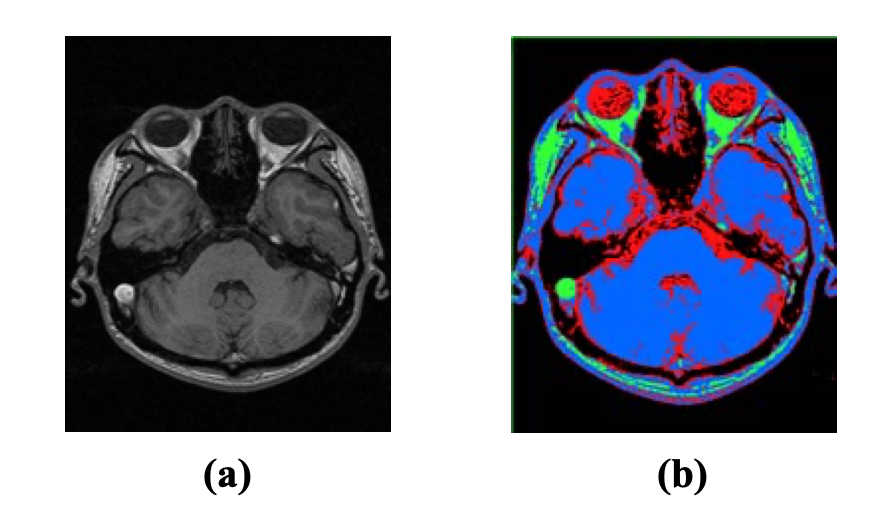
\includegraphics[width=175pt]{images/kmeans.png}
    \caption[K-Means clustering]{Original MRI head image (A) and the image after applying K-Means clustering (B) \cite{ng2006}}
    \label{fig:kmeans}
\end{figure}

\subsection{Fuzzy C-Means clustering}
Fuzzy C-Means clustering \cite{bezdek1981} is another algorithm which aims to solve the clustering problem. It is similar to K-Means as in the number of clusters is set by the user, and it is an iterative algorithm, which loops until some condition is met. 

However, Fuzzy C-Means is based on fuzzy logic. While in K-Means every data point belongs to exactly one cluster, 
in Fuzzy C-Means points can belong to numerous clusters to a certain degree. The membership grade for how strongly they belong to the cluster is between 0 and 1. It is important to point out that these values are not probabilities and do not need to add up to 1.

Fuzziness allows to incorporate uncertainty into our models. To understand what membership means, an example with temperatures is often used. Suppose we want to classify temperatures into groups of \textit{cold}, \textit{warm} and \textit{hot}. It is difficult to determine the threshold between cold and warm or warm and hot, because people perceive these things differently. 

In \ref{fig:fuzzy} the x-axis represents temperature and y-axis membership value. The vertical line is temperature \textit{t}. The membership value for \textit{t} in \textit{cold} is 0.8 which is ``fairly cold''. It is also 0.2 for \textit{warm} which might be interpreted as ``slighty warm''. The membership value for \textit{hot} is equal to 0, so \textit{t} can be considered ``not hot''.  

\begin{figure}[ht]
    \centering
    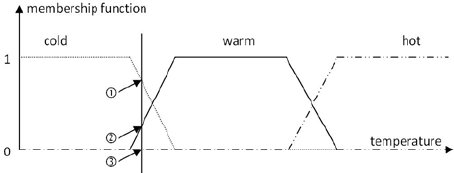
\includegraphics[width=250pt]{images/fuzzy.jpg}
    \caption{Fuzzy logic temperature sets}
    \label{fig:fuzzy}
\end{figure}

Similarly to K-Means, C-Means also aims to minimise an objective function:

\begin{equation}
\label{eq:objective-cmeans}
    J_{m} = \sum_{i=1}^{n}\sum_{j=1}^{c}u_{ij}^{m}\left \| x_{i} - c_{j} \right \|^{2}, 1\leq m\leq \propto 
\end{equation}

where \textit{$J_m$} is the objective function and \textit{m} is a real number which defines how \textit{fuzzy} the clustering should be. \textit{n} is the number of data points and \textit{c} is the number of fuzzy clusters. \textit{$u_{ij}^{m}$} is a membership value for point \textit{$x_i$} in the cluster \textit{$j$}. \textit{$\left \| x_{i} - c_{j} \right \|$} is a distance between a point and the cluster \textit{j} centroid.

The steps for this clustering algorithms are as follows:

\begin{enumerate}
  \item Assign random membership values to all data points for every cluster
  \item Compute the centroid for each cluster:
  
  \begin{equation}
    \label{eq:centroid-cmeans}
    c_{j} = \frac{\sum_{i=1}^{n}u_{ij}^{m} . x^{i}}{\sum_{i=1}^{n}u_{ij}^{m}}
    \end{equation}
    
   \item For each data point, recompute their membership values in the clusters:
   \begin{equation}
    \label{eq:update-cmeans}
    u_{ij} = \frac{1}{\sum_{k=1}^{c}\left ( \frac{\left \| x_i - c_j \right \|}{\left \| x_i - c_k \right \|} \right )^{\frac{2}{m-1}}}
    \end{equation}
    
    \item Repeat steps 2 and 3 until the membership values do not change by more than $\epsilon$, which is a pre-set value between 0 and 1
\end{enumerate}

The output of Fuzzy C-Means Clustering is a list of centroids and a partition matrix \textit{$w_{ij}$}, where each element is the membership value of the data point \textit{$x_i$} in the cluster \textit{$c_j$}. Finally, every point is assigned to the cluster for which it has the highest membership value.

FCM can be used for image segmentation in a similar manner as K-Means. 



\chapter{Computed Tomography}
\label{ch:ct}
Computed tomography was briefly mentioned in the previous chapter. Its invention had a huge impact on the field of diagnosis and rapidly increased in popularity over a few years. Compared to other techniques used in the 1970s, CT scans provided 3D visualisations with high detail.

In my thesis I am working with CT images, so in this chapter I am going to talk about the technology behind producing CT scans and the scans themselves.

%----SECTIONS----%
\section{Technology}
Technology behind CT scanning is based on X-Ray. X-Ray uses a tube in a fixed position which sends x-rays. In comparison to CT, where the tube moves around the patient in a so called translate-rotate motion. 

CT consists of an x-ray tube, which emits x-ray beams and an x-ray detector, which measures the x-ray transmission. The detector is located on the other side of the patient's body, just across from the tube. 

Patient's body can be divided into slices. You can imagine them as slices of bread. Thickness of these slices is determined by the thickness of the beam used for scanning. CT scanner performs the following steps on every slice. 

Both the tube and the detector move along the slice in one direction, performing a certain number of measurements. This phase is called translation. All the measurements collected during one translation phase are called a view. 

The rotation phase comes after every translation phase. The tube (together with the detector) rotates by 1°, so a view from a different angle can be obtained in the next translation phase. Hence, the name translate-rotate motion. After views for all the angles have been collected, the whole translate-rotate procedure is repeated on the next slice.

This is a basic principle of CT initially proposed by Haunsfield. His prototype called Mark I was able to collect 180 views over 180° (one view per 1° increment) and 160 measurements per view, which totalled in 28,800 measurements per whole scanning procedure. \cite{goldman2007}








\section{Scans}

CT scans are a reconstruction of the measurements collected during the scanning process. With their help, we can 'slice up the body' and look at what is inside in a non-invasive way. Slices are represented as a matrix called reconstruction matrix. These matrices consist of voxels - three-dimensional boxes. 

In \ref{fig:ct-brain-slices} you can see a number of axial (in the direction parallel to the body) slices of the human brain: 

\begin{figure}[ht]
    \centering
    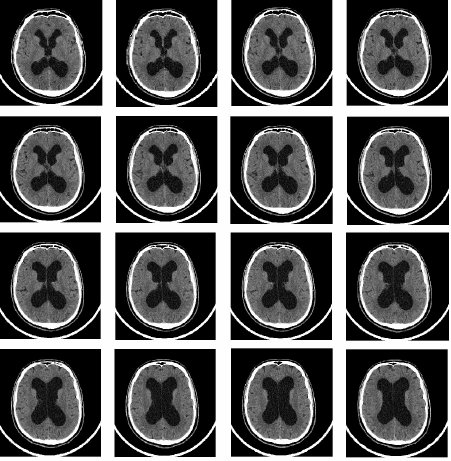
\includegraphics[width=200pt]{images/ct-brain-slices.jpg}
    \caption[CT brain slices]{CT brain slices \cite{brain-image}}
    \label{fig:ct-brain-slices}
\end{figure}

During the reconstruction phase, attenuation value for every voxel in the slice is assigned. Attenuation refers to loss of intensity of the ray passing through the tissue. These values can be computed by using simple algorithms like ART or Backprojection.

The attenuation values for every voxel are then transformed into Hounsfield units using this formula:

\begin{equation}
    \mathrm{CT number = [K \times (u_{voxel}-u_{water})]/u_{water}}
\end{equation}

\textit{K} is a constant nowadays set for 1000. \textit{$u_{voxel}$} and \textit{$u_{water}$} correspond to selected voxel's attenuation and water's attenuation respectively. This formula implies attenuation of water is 0 and the range of CT number is between -1000 and 1000. However, when it comes to images, we usually work with 256 greyscale values and the CT numbers need to be normalised. \cite{goldman2007}

\subsection{Artifacts}
CT scans are prone to artifacts. The reason for this is that a CT scan is computed from thousands of measurements. Any error in a measurement or computation of the voxel attenuation can be propagated to the image as an artifact. Basically, artifacts are attenuation values which do not correspond to the attenuation of the original tissue.

There are many ways in which an artifact can occur. Some of them stem from an incorrect position of the patient's body, physical processes occurring during data gathering or errors from reconstructing CT data. Artifacts can manifest themselves as streaks, shading, rings or distortion. They can be suppressed either on the side of CT manufacturers or by the operator \cite{barrett-keat2004}.  

\subsection{Formats}
There are two popular formats for storing CT and other medical images - DICOM and NIfTI. DICOM is a standard format scanners usually export the data in, whereas NIfTI is a more light-weighted format DICOM is typically converted to. 

DICOM is very complex and robust. With the introduction of CT, there was a need for ``a standard method for transferring images and associated information between devices manufactured by various vendors'' \cite{DICOM-spec}. Every object in the file is encapsulated in a tag. Objects store various types of information, for example data about the patient or the actual image data. Objects contain a tag (a two-number code, which defines the purpose of the object), VR (information about the data type), length of the data and in the end, the data itself \cite{neuro2016}.

NIfTI was firstly developed for use in neuroscience and with fMRI images specifically. The goal was to create a tool, that would be available for the whole research community, easy to use and suitable for a wide range of applications. NIfTI format is able to store not only data sets, but also for example statistical data. NIfTI files consist of a header and the actual data, either together in one .nii file, or separatly as .hdr and .img (header and image respectively) files. The header is 348 bytes long and its fields contain information about dimensionality, data type or data scaling. \cite{nifti} 

\subsection{Orientation}
When talking about medical images, it is important to know vocabulary related to directions. There are three axis describing 6 directions (Fig. \ref{fig:orientations}. Right and Left on the right-left axis correspond to the right and left directions. Anterior means towards front, posterior towards back. Inferior means below, towards the feet and superior means towards the head.

\begin{figure}[ht!]
    \centering
    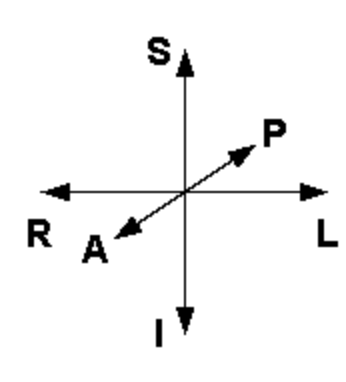
\includegraphics[width=150pt]{images/orientation.png}
    \caption[Orientations]{R - left to RIGHT, L - right to LEFT, A - posterior to ANTERIOR, P - anterior to POSTERIOR, I - superior to INFERIOR, S - inferior to SUPERIOR}
    \label{fig:orientations}
\end{figure}

Two popular coordinate systems are RAS and LAS. That means the first axis points to right (or left respectively), the second to anterior and the third to superior. RAS is a system used by neurologists and LAS by radiologists. 

We usually work with two spaces: scanner (world) space and voxel space. For the scanner space, the origin of the coordinate system is at the magnet isocentre. For voxel space, the origin is in the centre of the first voxel in the array. For example, if voxels are organised as RAS, it means voxels in rows are stored from left to right. Rows are stored from posterior to arterior to create a slice. And slices are ordered from inferior to superior to produce the whole image volume. It is possible to ``switch'' between these spaces using affine transformation. \cite{coordinate-systems}



\chapter{Convolutional Neural Networks}
\label{ch:cnn}
Convolutional Neural Networks have been around for some time, but gained popularity mostly in the recent years, since better hardware was available. It is a deep learning algorithm, mostly used on images. The tasks CNNs can solve include image classification or image segmentation and many others. Nowadays they are widely used for medical imaging problems. 

They were first introduced by Yann LeCun et al. in 1999 \cite{lecun1999}. They used CNN for recognising handwritten numbers. This classic dataset is known as MNIST. Underlying principles of convolutional neural networks are inspired by the visual system of cats - discovery of neurons responsive to different stimuli in different regions (receptive fields), which are then put together.

CNN is able to detect low-level features (for example edges) to high-level features (whole objects) in images. They are detected by applying appropriate filters. These filters are not pre-defined, but rather gained from training the network. To understand how this works, we need to introduce two important operations: convolution and pooling.

\textbf{Convolution} can be described as multiplication followed by summation. This operation is explained by the image \ref{fig:convolution-image}. Input for convolution is an image \textit{I}. Then we take a filter (or kernel) \textit{K} - which is a matrix of weights - and slide it through the image, computing convolutions for every position of the filter. Result \textit{I * K} is called a feature map. You can see the resulting feature map has smaller resolution than the original image. If we want to keep the original resolution, we can pad the original image around its edges. These filters are responsible for detecting features in images. CNNs usually do not consist of only one convolutional layer, so it is possible to detect high-level features. 

Another matrix operation is \textbf{pooling} (in \cite{lecun1999} originally referred to as sub-sampling). It is applied to feature maps from the previous convolutional layer. They down-sample (lower resolution of) feature maps, in order to reduce computation time, but also to allow for extracting more high-level features. There are two types of pooling, max and average pooling. Again, a filter passes through a feature map and returns the maximum and average respectively from its receptive field. This operation is visualised in \ref{fig:pooling-image}. In this image, stride of 2 was used. It means the filter did not pass the image pixel by pixel, but in ``steps'' of two.

\begin{figure}[ht]
    \centering
    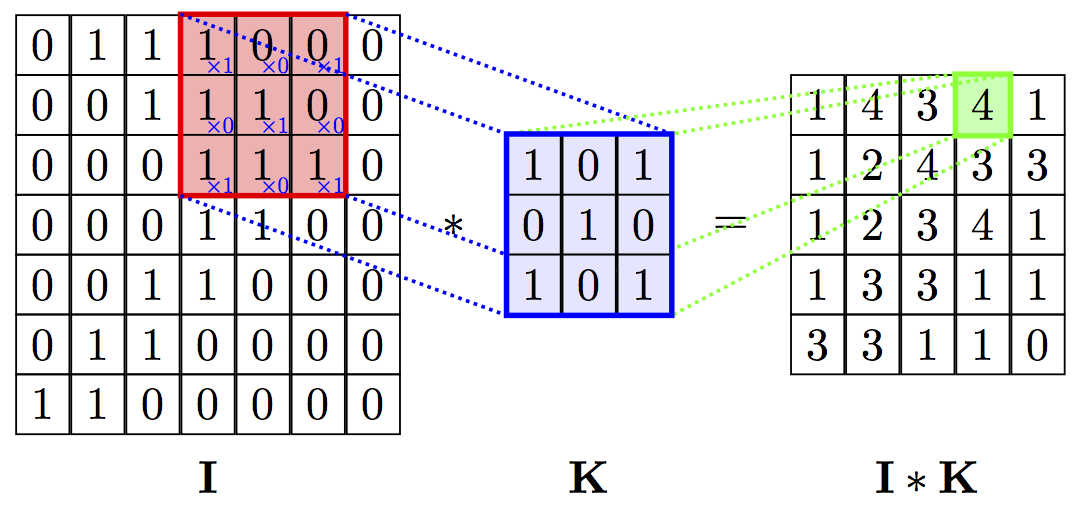
\includegraphics[width=200pt]{images/convolution-image.png}
    \caption{Visualisation of convolution}
    \label{fig:convolution-image}
\end{figure}

\begin{figure}[ht]
    \centering
    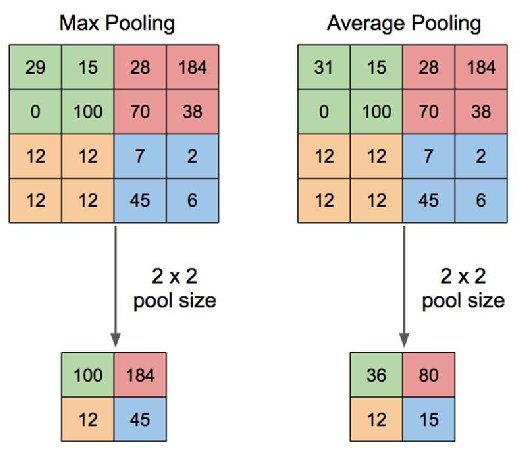
\includegraphics[width=200pt]{images/pooling.jpg}
    \caption{Visualisation of pooling}
    \label{fig:pooling-image}
\end{figure}

To see and understand how these layers work together, we can look at popular AlexNet \cite{alexnet2012} and its architecture \ref{fig:alexnet}. AlexNet won ImageNet classification competition in 2012, introducing an architecture which achieved a top-5 error of 15.3\%, which was 10\% lower than the second place.

Alex Krizhevsky used images of the volume of 224 x 224 x 3 (channels for RGB). These are fed to the first convolutional layer with 96 kernels of size 11 x 11 x 3. Every kernel produces one feature map, so the result is 55 x 55 x 96, which is then max-pooled and fed to the second convolutional layer. The second convolutional layer consists of 256 kernels of size 5 x 5 x 96, producing volume of 27 x 27 x 256, which is max-pooled again. The third layer contains 384 kernels of 3 x 3 x 256. Outputs (without max pooling) are sent to the fourth layer with 384 kernels of 3 x 3 x 384 and then to the fifth layer with 256 kernels of 3 x 3 x 384. Then two fully connected layers follow.

\begin{figure}[ht]
    \centering
    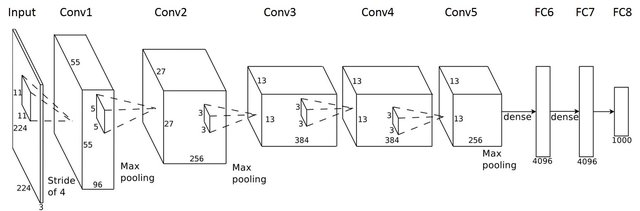
\includegraphics{images/alex-net.jpg}
    \caption[Architecture of AlexNet]{Architecture of AlexNet \cite{alexnet2012}}
    \label{fig:alexnet}
\end{figure}

Since 2012, CNNs have become very popular. There have been many extentions made to either solve problems occuring with CNNs or expand their use. I will talk about some of them next.

%----SECTIONS----%
\section{UNet}
The typical use of CNNs was mainly classification. The original architectures would usually just recognise what is on the image, but not where - which is the point of segmentation. In 2015, a new type of network for segmentation of biomedical images Unet was introduced \cite{unet2015}.

It is a FCV - fully convolutional network. That means there are no dense layers, only convolutions. This architecture (\ref{fig:unet}) consists of two parts or paths - \textbf{encoder} and \textbf{decoder}, which resembles the letter U. Hence, the name U-Net. Encoder serves for down sampling the high-resolution input image to a low-resolution output to find out what is in the image. Decoder up samples the low-resolution image back to the original resolution, retrieving locations of the features.

\begin{figure}[ht!]
    \centering
    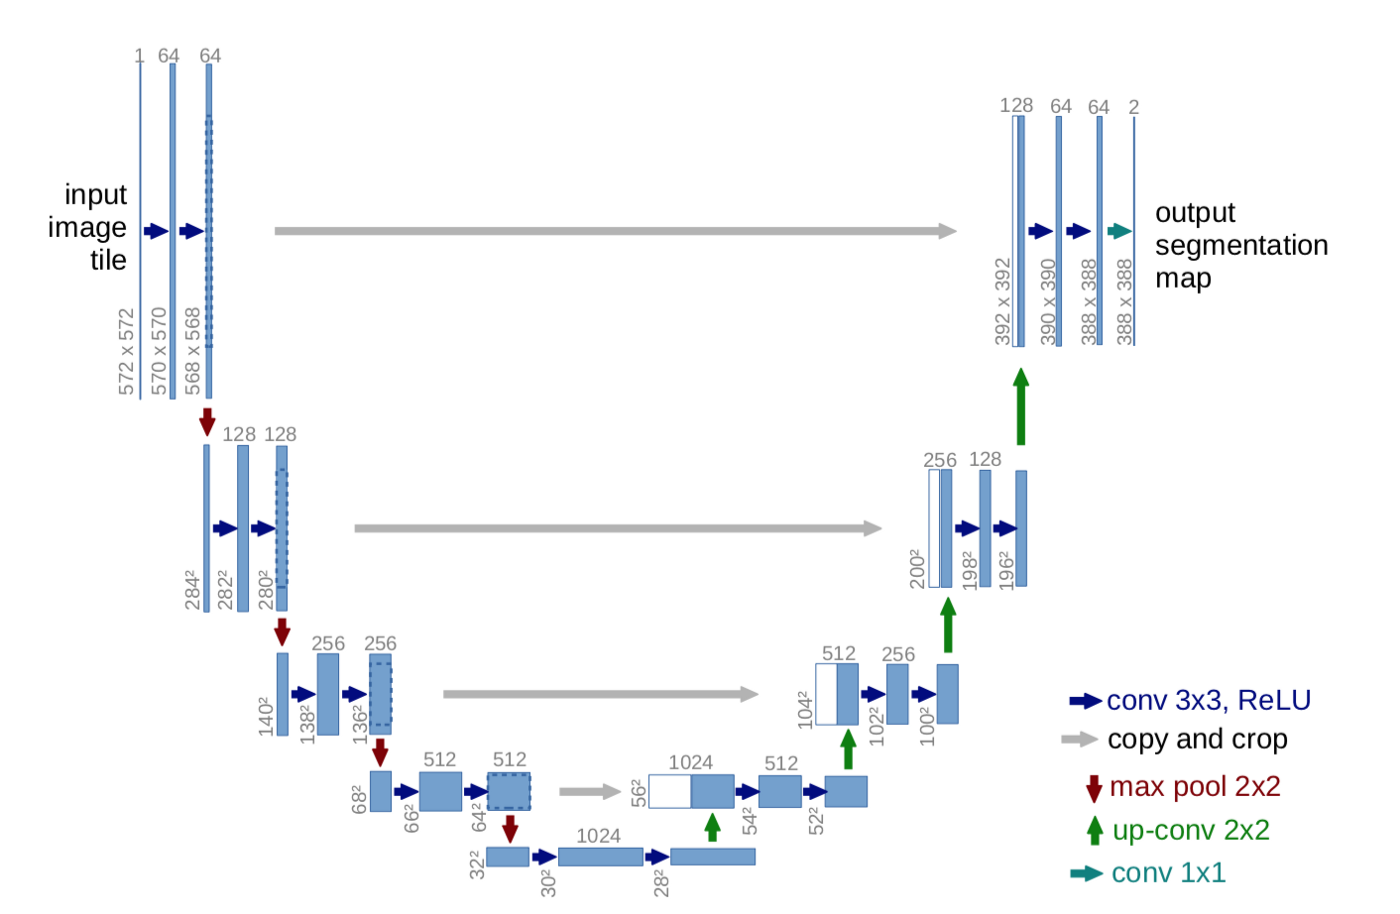
\includegraphics[width=300pt]{images/unet.png}
    \caption[Architecture of UNet]{Architecture of UNet \cite{unet2015}}
    \label{fig:unet}
\end{figure}

Encoder is a typical CNN, consisting of 3 blocks containing 2 convolutional layers followed by a max-pooling layer.

Decoder is more interesting. It is symmetrical to the encoder - 3 block consisting of up-convolution (transposed convolution) and 2 convolutions. The output is a predicted segmentation mask. Transposed convolution can be viewed as an operation opposite to convolution (but it is not the most precise definition). It creates a higher-resolution image from a low-resolution image. Furthermore, every result of up-convolution is concatenated with the feature map from the corresponding level in the encoder through skip connections. UNet has proven to perform very well on biomedical images.  

\pagebreak
\section{ResNet}
Another expansion built on CNNs is ResNet (Residual Network) \cite{resnet2016}, which succeeded in tackling issues with very deep networks. The general consensus was, the deeper the network is, the better performance it gives. However, it was observed, that training error for deeper networks gets higher than for their less deep counterparts. 

The degradation problem is caused by vanishing/exploding gradients. During backpropagation, multiplication of small (<1) and big (>1) numbers occurs. In deep networks, the multiplication takes place many times, causing it to get smaller and smaller until it vanishes or bigger and bigger until it blows up.

This problem can be solved by introducing residual blocks \ref{fig:res-block}. A skip connection is used to allow \textit{x} to be added to the output of later layers. This means, if vanishing gradient occurs, the network can be saved by ``going back'' to the previous layers. \ref{fig:resnet} shows a plain network and its counterpart (ResNet) with skip connections.

\begin{figure}[ht!]
    \centering
    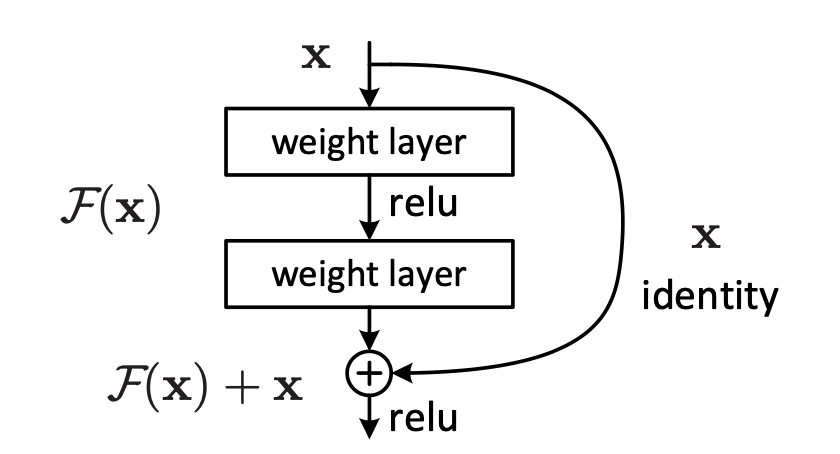
\includegraphics[width=130pt]{images/residual-block.png}
    \caption[Residual block]{Residual block \cite{resnet2016}}
    \label{fig:res-block}
\end{figure}

\begin{figure}[ht!]
    \centering
    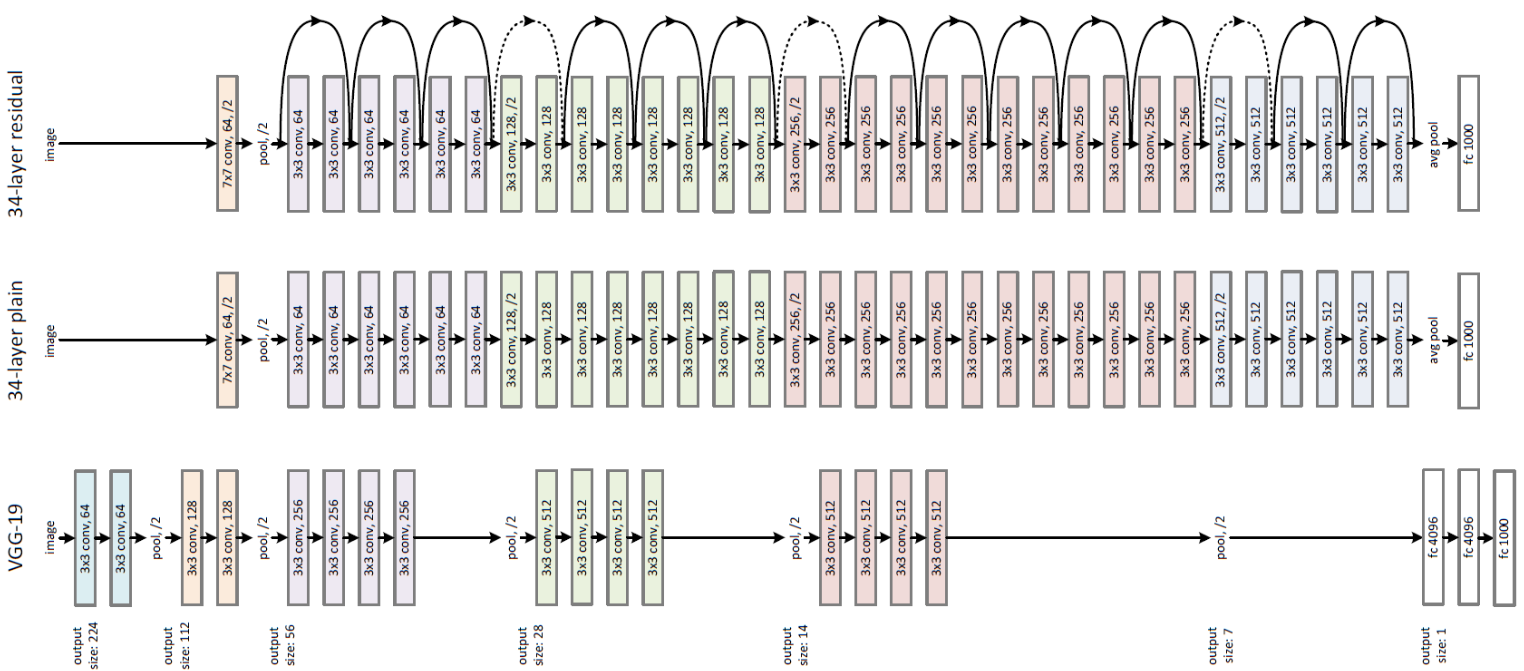
\includegraphics[width=350pt]{images/resnet.png}
    \caption[ResNet architecture]{ 34 layer ResNet (top), 34 layer plain network (middle), 19 layer VGG-19 (bottom)\cite{resnet2016}}
    \label{fig:resnet}
\end{figure}

\pagebreak
\section{DenseNet}
DenseNet \cite{densenet2017} was introduced in 2017. In an architecutre of this type, each layer receives ouputs from all the previous layers and then passes its input to all subsequent layers, to ensure maximum information flow.  In contrast to ResNet, where outputs are combined through summation, DenseNet uses concatenation.

Its name comes from the dense connectivity between layers. Suppose we have \textit{L} layers in the architecture. \textit{$l^{th}$} layer takes \textit{$l^{th}$} inputs (feature maps from previous layers) and its output goes to \textit{L} - \textit{$l^{th}$} following layers. This is illustrated in Figure \ref{fig:densenet}.

One of the improvements DenseNet brought, was a smaller amount of parameters to train, compared to traditional architectures or even ResNet. This feature makes it more computationally efficient. Dense layers have a few filters, which means, that the ``total'' number of feature maps passed through the network is rather small. The network then makes a decision based on all feature maps that appeared in it. Other advantages of DenseNets include memory efficiency. Furthermore, dense connections were observed to help with overfitting on small data sets.


\begin{figure}[ht!]
    \centering
    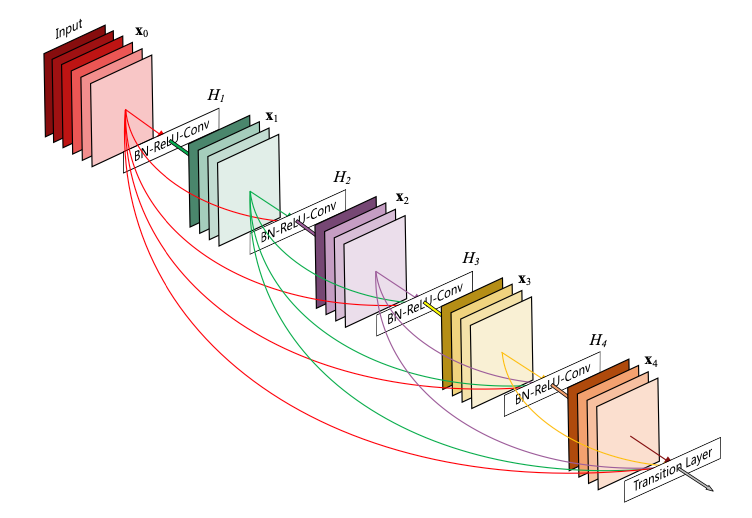
\includegraphics[width=200pt]{images/densenet.png}
    \caption[DenseNet architecture]{DenseNet architecture \cite{densenet2017}}
    \label{fig:densenet}
\end{figure}

\pagebreak
\section{R-CNN, Fast R-CNN, Faster R-CNN}
Previous architectures I was talking about served for solving classification (AlexNet, DenseNet, ResNet) or segmentation tasks (UNet). Another computer vision problem is object detection - finding instances of objects of classes in an image. That means localizing several objects of several classes withing one image.

R-CNN \cite{rcnn2014} (R stands for regions) proposed a method which combines region proposals and CNNs. Region proposals are a set of ``sub-images'' for classification. These regions are chosen by selective search. R-CNN architecture consists of 3 modules \ref{fig:rcnn}: First module takes the input image and generates around 2000 region proposals. These are then fed to a CNN which computes feature maps for them. And the last module is a linear SVM, which classifies the regions.

\begin{figure}[ht!]
    \centering
    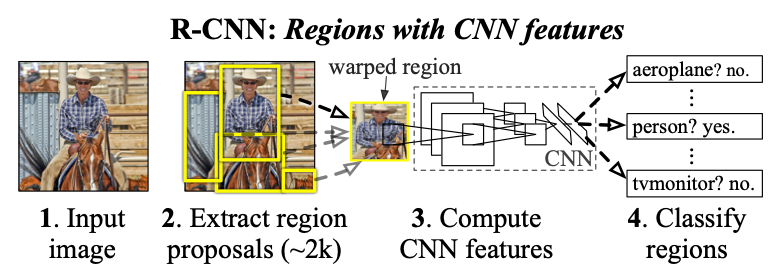
\includegraphics[width=200pt]{images/r-cnn.png}
    \caption[R-CNN modules]{R-CNN modules \cite{rcnn2014}}
    \label{fig:rcnn}
\end{figure}

The problem with R-CNN is that it is slow. This problem stems from the use of selective search to produce proposals, which are processed by CNN one by one . Therefore, its author came up with another method to speed up the process, Fast R-CNN \cite{fast-rcnn2015}. Input for this network is the whole image and a set of proposals. Generated convolutional maps are passed to the ROI (region of interest) pooling layer. This layer resizes them to a fixed size, so they can be fed into a fully connected layer. Squeezing an image and its proposals together reduces the number of convolutional passes and makes the whole process faster. 

Even faster version called Faster R-CNN was developed \cite{faster-rcnn2017}. Instead of using selective search to exhaustively produce region proposals, a Region Proposal Network is introduced. It is a fully convolutional network, which takes an image of any size as its input and outputs predictded object bounds. Those are then passed to the ROI pooling layer and then classified. 
\section{Capsule Network}
CNNs classify objects based on features they find in the image. When it spots a head, arms, legs and a body, it will classify the image as a person. However, spatial relationship between the features or their rotation is not considered. 

CapsNet \cite{capsnet2017} was developed to address this problem. A new neuron organisation called \textit{capsule} is proposed. Capsules are groups of neurons within one layer. Capsules output vectors (not scalars!), because they can encode more information. The size of the vector indicates the probability of the feature to even exist and its orientation describes various properties, like size, rotation, position, texture, etc. 

The proposed architecture (Fig \ref{fig:capsnet}) is quite simple. The first layer is convolutional and extracts features for capsules. The second layer is Primary Capsule layer. Consists of 32 capsules of 8 kernels and outputs 8D vectors. Those go to Digit Capsule Layer. This layer consists of 10 capsules (one capsule per class, in this case digits). All the capsules from the lower (primary) layer send their output to all the capsules in the higher (digit) level. The higher level outputs 16D vectors, which are fed to 3 fully connected layers. 

Dynamic routing is a process between two capsule layers. Its job is to replace max-pooling, during which spatial information is lost. Thanks to dynamic routing, output of one capsule gets send to the most appropriate parent capsule in the higher level. 

\begin{figure}[ht!]
    \centering
    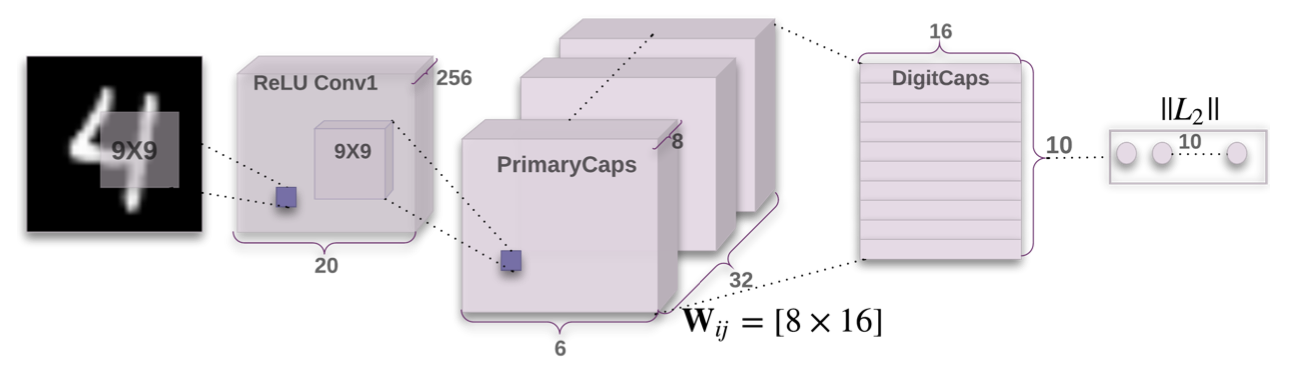
\includegraphics[width=300pt]{images/capsnet.png}
    \caption[CapsuleNetwork architecture]{CapsuleNetwork architecture \cite{capsnet2017}}
    \label{fig:capsnet}
\end{figure}

The model achieves very good results on classifying digits from MNIST and can also recognise overlapped digits in the MultiMNIST dataset. The way Capsule Networks work resembles human brain more than conventional CNNs. Even though they proved themselves successful on simple tasks like digit recognition, CapsuleNetworks are still a subject of research and need to improve their performance on more complex tasks. 





\chapter{Spine and vertebrae segmentation}
\label{ch:my-approach}
In this chapter I will describe the work I have done implementing neural nets for organs localisation in CT images. My task was to segment spine itself (binary segmentation task) and also specific vertebrae (multi-class segmentation task) from CT scans.

%----SECTIONS----%
\section{Keras}
The framework I used is called Keras \cite{keras}. It is a deep learning high-level API in python, which is built on top of either Theano or TensorFlow. It was built with the intent to provide a tool for quick prototyping and experimenting.

I used the TensorFlow \cite{tensorflow} backend.  TensorFlow is an open-source machine learning platform. Its abilities include: executing low level tensor operations on CPU, GPU and TPU, scaling computations to many devices or exporting to external runtimes.



\section{Data}
The data I used for this task was provided by the VerSe`19: Large Scale Vertebrae Segmentation Challenge \cite{verse1, verse2}. The dataset consists of 80 CT scans of human spines, together with a vertebrae segmentation mask for every scan, both in the NIfTI format. The original dataset also includes .png overview of the segmentation and vertebrae centroid annotations (for another task of the challenge, which is out of the scope of this thesis). There are also additional 40 scans without annotations. For loading and working with NIfTI files, I used library NiBabel \cite{nibabel}.

The voxel-level vertebral annotations were created manually by two neurologists. The spine segmentation masks were derived by me from the vertebral masks.

\begin{figure}[ht]
    \centering
    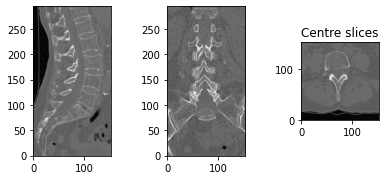
\includegraphics[width=250pt]{images/ct-sample.png}
    \caption[Sample data]{Saggital (side), coronal (frontal) and axial (horizontal) slices of a sample of the data}
    \label{fig:data-sample}
\end{figure}

\begin{figure}[ht]
    \centering
    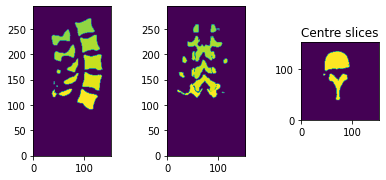
\includegraphics[width=250pt]{images/mask-sample.png}
    \caption{Vertebral segmentation mask of \ref{fig:data-sample}}
    \label{fig:mask-sample}
\end{figure}

\subsection{Spine}
Human spine consists of 24 vertebrae: C1-C7 (cervical spine), T1-T12 thoracic spine, L1-L5 lumbar spine. In very rare cases, an extra vertebrae L6 is present. Therefore, there are 26 classes in the data: background class [0] and vertebrae [C1-L6] which correspond to values [1-25] in the mask. Figure \ref{fig:vertebrae-annotations} shows annotations for [T2-L5].

\begin{figure}[ht]
    \centering
    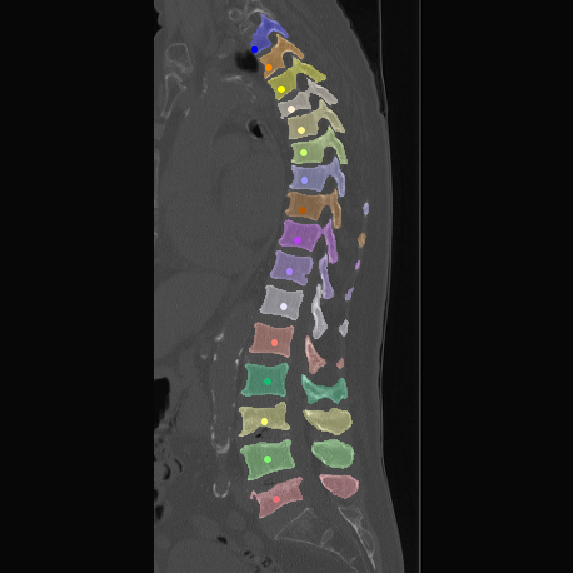
\includegraphics[width=150pt]{images/vertebrae-annotations.png}
    \caption{Vertebrae [T2-L5]}
    \label{fig:vertebrae-annotations}
\end{figure}

\subsection{Data characteristics}
One of the most important things about images when using neural networks is their size. In this dataset, images have various sizes in all dimensions, various ratios. The sizes range from as small as (57, 175, 175) to as big as (121, 915, 1189). Voxels do not store values typical for images (0-255), but attenuation values for the specific voxels. These vary all around the data set from -2290 (air) to 4106 (bones or metals). Voxels of the CT scans are also stored in various orientations: LAS, PIR, LPS and PSR.

Not all images contain the whole spine, usually it is some subset of vertebrae. This means, some of the vertebrae occur throughout the data set more often than others. [C1-C7] are underrepresented with less than 20 occurencies, [T1-T12] occur on average 35 times and the third group of vertebrae [L1-L5] is represented with more than 60 instances per vertebrae. The special L6 appears only in 2 scans from the whole dataset.

The dataset is imbalanced not only because of that, but also because different vertebrae cover different volumes. To put it easily, the background class is voxel-wise the most common class among the data. It accounts for more than 97\% of all voxels, the remaining 3\% is the spine. Also each vertebrae type accounts for less than 0.5\%. 


\section{Preprocessing}
Since the data contains attenuation values, initially I normalised it to (0,255), the common grey scale value range, so it could be easier to work with. Neural nets usually accept inputs of the same dimensions, so I resized my samples to dimensions of (96, 96, 128). The dataset consists of only 80 scans in different orientations, so it was important to put them into a common orientation. I chose RAS, as it is widely used around the community. For the reorienting, I used library called Nipype\cite{nipype}. Apart from resizing, I also implemented cropping and padding with zeros for 3D images, which I did not use in the end.

All the preprocessing took place prior to training and the data was saved to the disc in the .npy format. This way a lot of time during the training was saved. 
\section{3D UNet}
\begin{figure}[ht!]
    \centering
    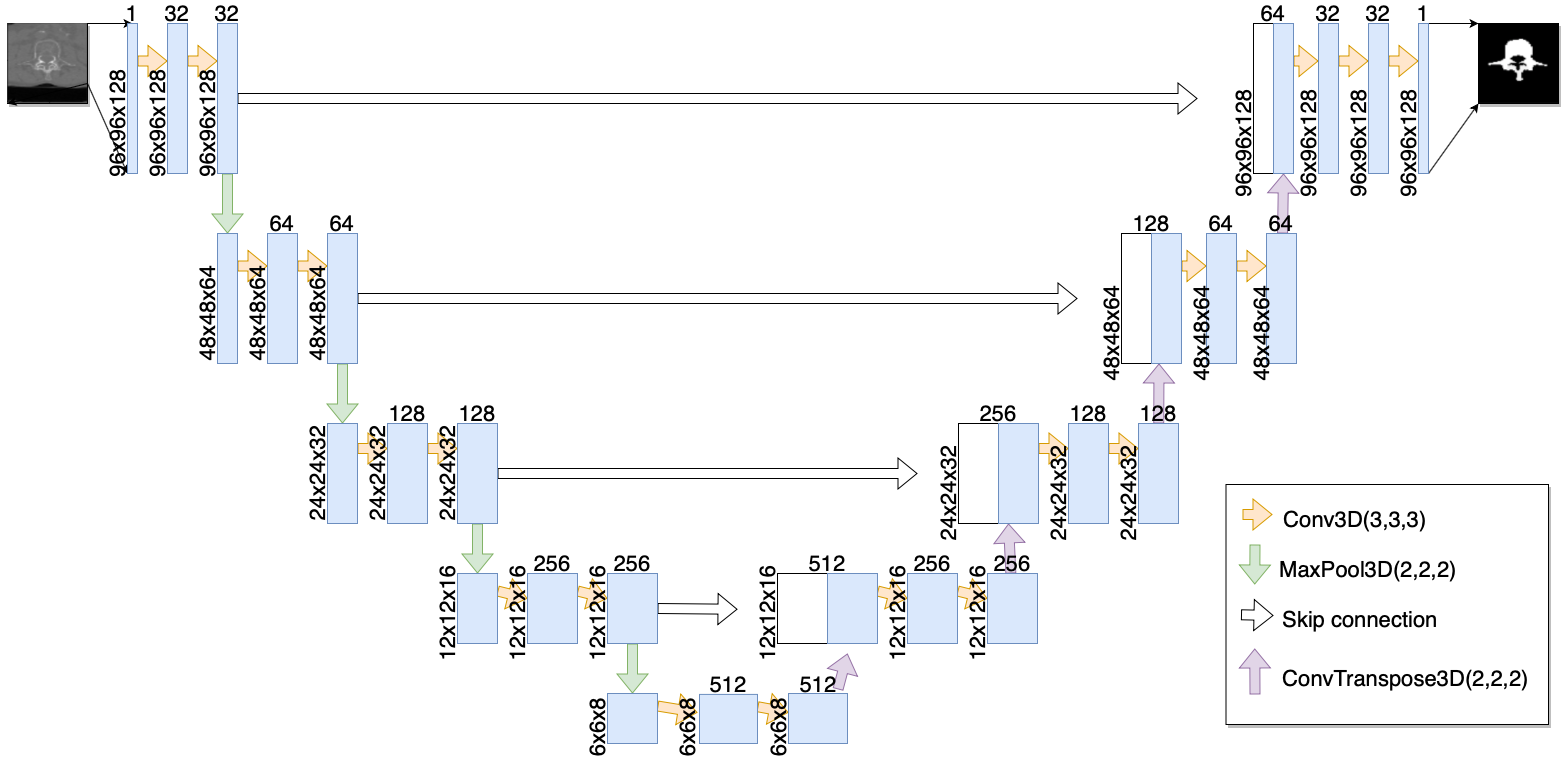
\includegraphics[width=1.\textwidth]{images/unet3d.png}
    \caption{3D UNet architecture}
    \label{fig:3D-unet}
\end{figure}

My architecture \ref{fig:3D-unet} is based on the original architecture of UNet \cite{unet2015} and Ultrasound Nerve Competition Tutorial \cite{jocic}. It is an encoder-decoder with skip connections between the same levels  of the contracting and the expansive path. The major difference is that my network accepts 3D images and also produces 3D outputs. Furthermore, all the operations: convolution, maxpooling and up-convolution are changed to work in the three-dimensional space. 3D filters used are: (3,3,3) for convolution, (2,2,2) for maxpooling and (2,2,2) for up-convolution. These filters ``slide'' through the image in all three dimensions, meaning they are capable of taking the third dimension into account and recognising features in the 3D context. Overview for the number of filters in each layer is in Table \ref{tab:neurons}.

Input to my network is of the size 96x96x128. There are 5 levels (Table \ref{tab:encoder-block}) in the architecture. Starting with the contracting path, the first level consists of 2 3Dconvolutions, 32 filters each, followed by ReLU. The output is then downsampled by 3Dmaxpooling, reducing its size by half. The number of convolutional filters doubles with each level, also doubling the number of 3D feature vectors. 

%up
The expanding path (Table \ref{tab:decoder-block}) starts by a 3Dup-convolution from the bottom level. This operation doubles the output resolution and also reduces the number of feature maps. These are then concantated with its counterpart feature maps from the contracting path. Then, again, 2 3Dconvolutions follow. The number of convolutional filters reduces by half on the way up. 

On the top of the expanding path, we are back to the original resolution of the input image. The very last convolutional layer depends on the task. For binary segmentation, the last layer consists of 1 (1,1,1) filter and sigmoid activation, outputting a volume of 96x96x128 with probabilities for whether the voxel belongs to the foreground class.

For multiclass segmentation, the last convolutional layer consists of 26 (1,1,1) filters (one for each class), with softmax as the activation function. The size of the output is 96x96x128x26, where probabilities for every voxel for belonging to each class a stored. 

%---------------------------------------------------------------

\begin{table}[]
\centering
\begin{tabular}{@{}ccc@{}}
\toprule
\multicolumn{1}{l}{Encoder layers} & \multicolumn{1}{l}{Decoder layers} & \multicolumn{1}{l}{Neurons} \\ \midrule
1, 2                               & 17, 18                             & 32                          \\
3, 4                               & 15, 16                             & 64                          \\
5, 6                               & 13, 14                             & 128                         \\
7, 8                               & 11, 12                             & 256                         \\
\multicolumn{2}{c}{9, 10}                                               & 512                         \\ \bottomrule
\end{tabular}
\caption[Number of neurons for each layer]{Number of neurons in 3D Convolutional layers. Layers 9 and 10 represent the bottom of the network. Numbering starts at with the first convolutional layer of the network and ends with the last layer before the output layer.}
\label{tab:neurons}
\end{table}

%---------------------------------------------------------------

\begin{table}[]
\centering
\begin{tabular}{@{}ccccc@{}}
\toprule
Layer          & Filter size & Strides & Padding & Activation \\ \midrule
3D Convolution & 3, 3, 3     & 1, 1, 1 & same    & ReLu       \\
3D Convolution & 3, 3, 3     & 1, 1, 1 & same    & ReLu       \\
3D MaxPooling  & 2, 2, 2     & 2, 2, 2 & same    &            \\ \bottomrule
\end{tabular}
\caption{Encoder block}
\label{tab:encoder-block}
\end{table}

%---------------------------------------------------------------

\begin{table}[]
\centering
\begin{tabular}{@{}ccccc@{}}
\toprule
Layer                     & Filter size & Strides & Padding & Activation \\ \midrule
3D Transposed Convolution & 2, 2, 2     & 2, 2, 2 & same    &            \\
3D Convolution            & 3, 3, 3     & 1, 1, 1 & same    & ReLu       \\
3D Convolution            & 3, 3, 3     & 1, 1, 1 & same    & ReLu       \\ \bottomrule
\end{tabular}
\caption{Decoder block}
\label{tab:decoder-block}
\end{table}





\section{Spine segmentation}

\subsection{Loss functions}
One of the most important things to get good results with neural networks is to choose a suitable loss function. Loss function measures how well the network's predictions are during training. The goal of the network is to minimise its value. Some of them lead to convergence of the network, some of them do not.

There are numerous loss functions used for image segmentation. Since my data is very unbalanced, some losses were more suitable than the others. Badly chosen loss with unbalanced data can lead to predicting only zeros (only background). I chose 2 and compared their performance.

One of the losses that perform well on unbalanced data is Dice loss. It is an overlap measure. Instead of evaluating every pixel (voxel) independently, Dice looks at how well the ground truth and the prediction overlap. This means that if half of a small object and half of a large object are detected, the loss will be the same.

Another loss function I used is binary crossentropy. To put it simply, a negative logarithm for every prediction is computed. This means that if the prediction for the object pixel is 1, loss will be also 1. And similarly, for very low predictions logarithm gets bigger and bigger. This loss on itself does not deal with class imbalance. For this reason I computed class weights and multiplied the crossentropy results by them, making the spine object ``more important'' than the background. By using this loss I tried to solve the gradient exploding and instability issues I encountered with Dice loss - I can say they did not occur with binary crossentropy.

\subsection{Training}
The size of the dataset is 80 scans. The data was split in the ratio of 80/10/10, which means 64 scans were used for training, 8 for validation and 8 for testing. The data was sorted in the same order as it was originally in the dataset, no special selection of the split. I chose this ratio, as the dataset is rather small and I wanted to reserve as many examples for training as I could. The algorithm ran on a Cloud TPU with 35GB RAM offered by Google Colab. Models were trained for 40 epochs, which took approximately 10 hours. 

I will be comparing 2 models, one trained with binary crossentropy loss (Model 1) and Dice loss (Model 2). Both were trained with stochastic gradient descent - this means the batch size was 1 and weights were updated for each example of the training set. This approach proved to be considerably faster than the mini-batch approach (8 batches). Input images were normalised to the range (0,1). 

Model 1 was trained with Adam optimizer, \textit{learning\_rate}=0.0001, \textit{beta\_1 = 0.9}, \textit{beta\_2 = 0.999}. Choosing parameters for Model 2 with Dice loss was more difficult, exploding gradients occurred frequently. Learning rates for Adam optimizer I tried include: 0.001, 0.00015, 0.0001, 0.000015, 0.00001 and 0.000001. I settled for \textit{learning\_rate} = 0.00001 together with clip\_norm = 1. and clip\_value = 0.5 (to prevent exploding/vanishing gradients) as it was one of the few settings to yield reasonable results. \textit{beta\_1 = 0.9} and \textit{beta\_2 = 0.999} are the same as with Model 1.

\subsection{Metrics}
Often it is difficult to choose the metric that best represents how good our results are. Therefore I chose 4 different metrics, where each of them takes into account different things. In the following equations, \textit{TP} stands for true positive, \textit{TN} for true negative, \textit{FP} for false positive and \textit{FN} for false negatives.

Pixel wise accuracy (Eq. \ref{eq:pixel-wise-accuracy}) is a metric that simply measures the percentage of correctly classed pixels. However, this metric gives good results also for images with very small objects, even though they are not classified properly.

\begin{equation}
\label{eq:pixel-wise-accuracy}
    \textup{pixel wise accuracy}  = \frac{TP + TN}{TP + TN + FP + FN} 
\end{equation}

Dice coefficient (Eq. \ref{eq:dice-accuracy}) was explained before. It measures overlap between the ground truth and predicted object. 

\begin{equation}
\label{eq:dice-accuracy}
    \textup{dice coefficient}  = \frac{2TP}{2TP + FP + FN} = \frac{2|X\cap Y|}{|X|+|Y|}
\end{equation}

Intersction over Union (IoU) (Eq. \ref{eq:iou-accuracy}) is very similar to Dice. It measures overlap as well, but penalizes wrong predictions more than Dice. 

\begin{equation}
\label{eq:iou-accuracy}
    \textup{IoU}  = \frac{TP}{TP + FP + FN} = \frac{2|X\cap Y|}{|X|+|Y| - |X\cap Y|}
\end{equation}

The last metric AUC-ROC Curve (Area under Curve - Receiver Operating Characteristics curve) is a metric that measures how well the model can separate classes. Value 0.5 means it cannot distinguish between classes at all.   

\subsection{Results}
Results for all 4 metrics for Model 1 and Model 2 are in Table \ref{tab:results-spine}. Predictions were thresholded at 0.9. Model 2 performed significantly better in all metrics except for AUC-ROC, which means it is worse at separating classes. 

Sample predictions and segmentations are in Fig. \ref{fig:spine-segmentations} and more in the appendix. We can see that predictions with Model 2 (with Dice loss) are very tightly around the spine, have smooth edges. There are a lot of false negatives, as the model seems to be trying to not class background as foreground. Model 1 (with weigthed binary crossentropy), on the other hand, is able to spot more details and irregularities. However, for the price of false positives, when it often detects areas outside of the object. The weighted binary crossentropy ensured that pixels are not easily classed as the background.

For cross validation and comparison with another architecture, I chose Model 2 (or rather its hyper-parameters and validation loss), as it outperformed Model 1 in almost all metrics. Furthermore, as you can see in Fig. \ref{fig:spine-losses}, performance of Model 2 was consistently getting better, while Model 1 seemed to have reached its best at around the 20th epoch, with validation loss not getting much better since. It was only train loss which was decreasing, meaning the model was overfit.  

\begin{figure}
\begin{subfigure}{.5\textwidth}
  \centering
  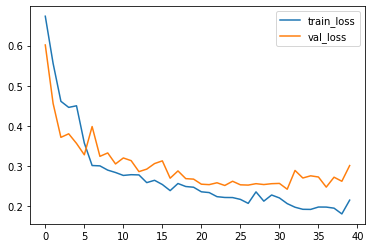
\includegraphics[width=.8\linewidth]{images/loss-binary.png}
  \caption{Model 1}
  \label{fig:sfig1}
\end{subfigure}%
\begin{subfigure}{.5\textwidth}
  \centering
  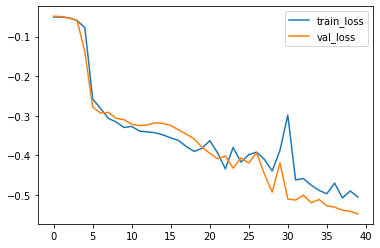
\includegraphics[width=.8\linewidth]{images/loss-dice.png}
  \caption{Model 2}
  \label{fig:sfig2}
\end{subfigure}
\caption[Loss over epochs for Model 1 and 2]{Validation and training loss over 40 epochs for Model 1 and 2. X axis represents number of epochs, Y axis is loss.}
\label{fig:spine-losses}
\end{figure}


To ensure generalisation, I performed 3-fold cross validation on 72 samples. Since training the network is very time consuming, I decided to cross validate the network only on 20 epochs. The folds were chosen randomly. Results, again for all four metrics, are in \ref{tab:cross-val-spine}. Even after only 20 epochs, the results are generally better than for Model 1 after 40 epochs. Small standard deviations also suggest, that accuracy did not change much across the folds.


The idea behind my architecture is that 3D convolutions should be better at  extracting features from 3D volumes, because they can ``capture'' the third dimension. Therefore, I compared my model with the corresponding 2D one. The input were 96x96 axial slices of the spine. Hyper-parameters and validation loss for training were the same as for Model 2, except for the batch size, which I set to 32, which is a widely used value. The number of epochs was 40 and the training took only 3.5 hours. Results are in Table \ref{tab:results-spine-2D}. Both the models yielded similar results, with UNet 2D being slightly better, but not significantly. Comparison of segmentations is in Fig. \ref{fig:unet2D-spine}. UNet 2D was able to capture more details and edges than UNet 3D. 





%-------------------------------------------------------------------

\begin{figure}[ht!]
\centering
\begin{subfigure}[b]{0.70\textwidth}
   \includegraphics[width=1\linewidth]{images/results_1/original.png}
   \caption{Original image}
   \label{fig:Ng1} 
\end{subfigure}

\begin{subfigure}[b]{0.70\textwidth}
   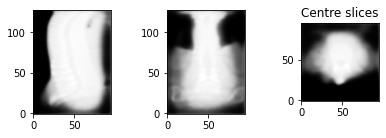
\includegraphics[width=1\linewidth]{images/results_1/binary_mask.png}
   \caption{Predictions of Model 1}
   \label{fig:Ng2}
\end{subfigure}

\begin{subfigure}[b]{0.70\textwidth}
   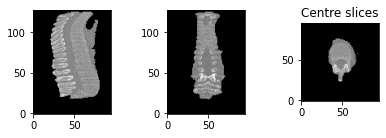
\includegraphics[width=1\linewidth]{images/results_1/binary_segmented.png}
   \caption{Segmented image with Model 1}
   \label{fig:Ng3}
\end{subfigure}

\begin{subfigure}[b]{0.70\textwidth}
   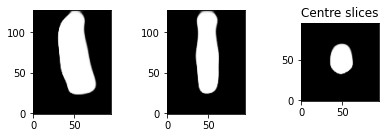
\includegraphics[width=1\linewidth]{images/results_1/dice_mask.png}
   \caption{Predictions of Model 2}
   \label{fig:Ng4}
\end{subfigure}

\begin{subfigure}[b]{0.70\textwidth}
   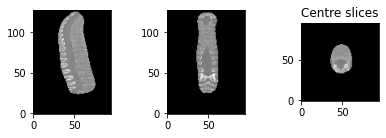
\includegraphics[width=1\linewidth]{images/results_1/dice_segmented.png}
   \caption{Segmented image with Model 2}
   \label{fig:Ng5}
\end{subfigure}

\caption[Results of spine segmentation]{Original and segmented CT image of a spine using Model 1 and Model 2.}
\label{fig:spine-segmentations}
\end{figure}

%---------------------------------------------------------------

\begin{table}[ht!]
\centering
\begin{tabular}{@{}ccc@{}}
\toprule
Metric                  & Model 1    & Model 2   \\ \midrule
Pixel wise accuracy     & 0.90773034 & 0.9738508 \\
Dice coefficient        & 0.36018768 & 0.6070875 \\
Intersection over union & 0.21965213 & 0.435841  \\
Area under ROC          & 0.9219055  & 0.8547937 \\ \bottomrule
\end{tabular}
\caption[Comparison of Model 1 and 2]{Comparison of Model 1 and Model 2. Metrics used: pixel wise accuracy, Dice coefficient, intersection over union and area under ROC}
\label{tab:results-spine}
\end{table}

%---------------------------------------------------------------

\begin{table}[ht!]
\centering
\begin{tabular}{@{}cc@{}}
\toprule
Metric                  & 3D UNet                 \\ \midrule
Pixel wise accuracy     & 0.959435(+/- 0.010288)  \\
Dice coefficient        & 0.397100 (+/- 0.008332) \\
Intersection over union & 0.247772 (+/- 0.006509) \\
Area under ROC          & 0.730441 (+/- 0.038218) \\ \bottomrule
\end{tabular}
\caption[3-fold Cross validation] {Results of 3-fold cross validation after 20 epochs with 3D UNet, standard deviation included. Evaluated with 4 different metrics: pixel wise accuracy, Dice coefficient, intersection over union and area under ROC}
\label{tab:cross-val-spine}
\end{table}

%---------------------------------------------------------------

\begin{figure}[ht!]
\centering
\begin{subfigure}[b]{0.70\textwidth}
   \includegraphics[width=1\linewidth]{images/results_3/original.png}
   \caption{Original image}
   \label{fig:Ng1} 
\end{subfigure}

\begin{subfigure}[b]{0.70\textwidth}
   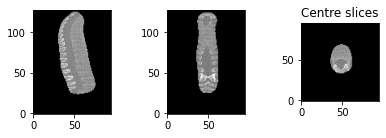
\includegraphics[width=1\linewidth]{images/results_3/3D.png}
   \caption{Segmented image with 3D UNet}
   \label{fig:Ng2}
\end{subfigure}

\begin{subfigure}[b]{0.70\textwidth}
   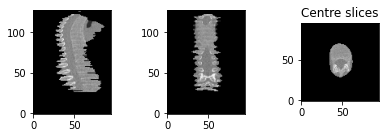
\includegraphics[width=1\linewidth]{images/results_3/2D.png}
   \caption{Segmented image with 2D UNet}
   \label{fig:Ng3}
\end{subfigure}

\caption[Comparison UNet 3D and UNet 2D]{Original and segmented CT image of a spine using Model 1 and Model 2. Threshold for predictions is 0.9.}
\label{fig:unet2D-spine}
\end{figure}

%---------------------------------------------------------------

\begin{table}[ht!]
\centering
\begin{tabular}{@{}ccc@{}}
\toprule
Metric                  & UNet 2D    & UNet 3D   \\ \midrule
Pixel wise accuracy     & 0.97514015 & 0.9738508 \\
Dice coefficient        & 0.6125695 & 0.6070875 \\
Intersection over union & 0.44151428 & 0.435841  \\
Area under ROC          & 0.8458461  & 0.8547937 \\ \bottomrule
\end{tabular}
\caption[UNet 2D and UNet 3D results]{Comparison of results from 3D and 2D UNet using metrics: pixel wise accuracy, Dice coefficient, intersection over union and area under ROC}
\label{tab:results-spine-2D}
\end{table}

\subsection{Summary}
I managed to get good results with the 3D UNet network. The spine is correctly located in the images. However, still unable to detect space inbetween vertebrae. There is a potential to improve performance by training the model for more epochs, because the loss was still steadily improving. Cross validation results proved the model can generalise well for the given dataset. However, the 3D architecture did not bring any improvement compared to the 2D one, as the results were very similar, with 2D one slightly outperforming the 3D one. 
\section{Vertebrae segmentation}
\subsection{Loss functions}
For multi-class segmentation tasks, different losses are needed. In the case of segmenting specific vertebrae,  the class imbalance is even worse than with the whole spine. 

There is a special type of Dice loss - soft Dice loss, which computes loss for every class separately and then computes the mean. This should work well with small object, as Dice loss does. 

Another loss I was considering was categorical crossentropy loss, which is a generalised version of binary crossentropy for more than 2 classes. I was planning on applying class weights to this loss as well, but unfortunately, Keras does not provide this feature for 2D and 3D volumes. Therefore I focused on the soft Dice loss.

\subsection{Training}
Very similarly to the spine segmentation, I used data split 80/10/10 resulting in 64 training examples, 8 for validation and 8 for testing. It ran on the Google Colab's TPU for 10 hours for 40 epochs. 

The model was trained with soft Dice loss and Adam optimizer, with \textit{learning\_rate}=0.00001. \textit{beta\_1}=0.9, \textit{beta\_2}=0.999 were set by default by the optimizer. The batch size was set to 1 to speed up the training.

In contrast to spine segmentation, the input masks were one-hot-encoded and had dimensions of 96x96x128x26 (26 is the number of classes), where each of the 26 channels represents a segmentation mask for one class. The network outputs a volume of the same dimensions, with probabilities of the pixels to belonging to each of the classes. Probabilities across all classes for one pixel sum to 1. This output is then sent through the argmax function to determine the class (channel) with the highest probability. The result is a segmentation mask of 96x96x128x1, where each element contains the class number. 

\subsection{Results}
The network seemed to be unable to train properly for this task and chosen parameters. The loss would be decreasing for a few epochs, but then got stuck and stayed the same till the rest of the training. I tried overfitting the network only on one image, changing learning rates in the range from 0.001 to 0.000001, with not much success. The losses are in Fig. \ref{fig:loss}. Output of the network was almost all zeros, with a few pixels classified as a vertebrae class. 

\begin{figure}[ht!]
    \centering
    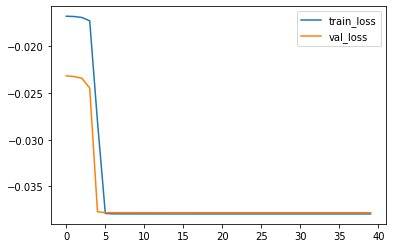
\includegraphics[width=250pt]{images/plot_loss.png}
    \caption[Validation loss]{Validation and train loss across 40 epochs. X axis is number of epochs, Y axis is loss.}
    \label{fig:loss}
\end{figure}

I tried running 2D UNet with the same parameters (only batch size set to 32) to see, if the network is able to learn something, but the results were the same. Loss was decreasing at the beginning, but later stayed the same until the last 40th epoch.

\subsection{Summary}
My network could not be trained for multi-class segmentation problems in either 3D and 2D version. I suspect the problem lays in the choice of the loss function, as it did not work for either of the architectures and the same problem occured for different learning rates. To improve the performance, I could try the before mentioned categorical crossentropy, even though it does not take into account class imbalance. Another approach that could be used is extracting single vertebrae from the images for training.  









%----MY APPROACH----%
\setsecnumdepth{part}
\chapter{Conclusion}
\label{ch:conclusion}
I started my thesis with the literature review, where I covered the history of medical imaging and classical methods for image analysis, which were popular in the pre-ML era. I focused on CT images, the technology and other specifics of this medium. I researched convolutional neural networks and their extensions for different purposes.

The practical part covered implementing a CNN model for segmentation of a spine and specific vertebrae. The CT data underwent preprocessing to make it suitable for this task. My architecture was based on UNet, but modified to handle CT images (3D volume). I compared the performance of my 3D model with the original 2D model on 3D images. I managed to segment the spine with satisfactory results. However, for specific vertebrae I could not make the network perform well. The results show, the derived architecture did not achieve better performance on the chosen dataset. In fact, it was slightly outperformed. 

I am satisfied with my results, as this is the first time I worked with CNNs. However, there are still many ways on how to improve/change the architecture or other tasks that can be done with this data. Automatic segmentation of the spine or vertebrae can be used by doctors to give better diagnosis to their patients.


\begin{thebibliography}{9}

\bibitem{glasser1993}
GLASSER O., \textit{Wilhelm Conrad Röntgen and the Early History of the Roentgen Rays} [online]. San Francisco: Norman Publishing, 1993. [Accessed 27 April 2020]. ISBN 0-930405-22-6. Available from: https://books.google.sk/books?id=5GJs4tyb7wEC

\bibitem{bhattacharyya2016}
BHATTACHARYAA K. B., Godfrey Newbold Hounsfield (1919–2004): The man who revolutionized neuroimaging. \textit{Ann Indian Acad Neurol.} [online]. October-December 2016, 19(4), pp. 448-450. [Accessed 27 April 2020]. ISSN 1998-3549. Available from: doi:10.4103/0972-2327.194414

\bibitem{lauterbur1973}
LAUTERBUR P.C., Image Formation by Induced Local Interactions: Examples Employing Nuclear Magnetic Resonance. \textit{Nature} [online]. March 1973, 242, pp. 190-191. [Accessed 27 April 2020]. ISSN 1476-4687. Available from: https://www.biac.duke.edu/education/courses/fall05/fmri/readings/
week3/1973\_Nature\_Lauterbur.pdf

\bibitem{eurostat2019}
Medical technologies - examinations by medical imaging techniques (CT, MRI and PET). In: \textit{EUROSTAT} [online]. European Union 2019. [Accessed 27 April 2020]. Available from: https://ec.europa.eu/eurostat/web/products-datasets/-/hlth\_co\_exam

\bibitem{wells2016}
WELLS W.M., Medical Image Analysis – past, present, and future. \textit{Medical Image Analysis} [online]. October 2016, 33, pp. 4-6. [Accessed 27 April 2020]. ISSN 1361-8415. Available from: doi: doi.org/10.1016/j.media.2016.06.013

\bibitem{thresholding}
SAHOO P.K., SOLTANI S., WONG A.K.C, A survey of thresholding technique. \textit{Computer Vision, Graphics, and Image Processing} [online]. 1988, 41(2), pp. 223-260. [Accessed 7 May 2020]. ISSN 0734-189X. Available from: http://www.sciencedirect.com/science/article/pii/0734189X8890022

\bibitem{medical-imaging-handbook}
BANKMAN I.N., \textit{Handbook of Medical Image Processing and Analysis}. London: Academic Press, 2000 ISBN 0-12-077790-8. 

\bibitem{otzu1979}
OTZU N., A Threshold Selection Method from Gray-Level Histograms. \textit{IEEE Transactions on Systems, Man, and Cybernetics} [online]. 1979, 9(1), pp. 62-66. [Accessed 30 April 2020]. ISSN 2168-2909. Available from: doi: 10.1109/TSMC.1979.4310076

\bibitem{clustering}
JAIN A.K., DUBES R.C., \textit{Algorithms for clustering data} [online]. Englewood Cliffs: Prentice-Hall, Inc., 1988. [Accessed 7 May 2020]. ISBN 978-0-13-022278-7. Available from: https://homepages.inf.ed.ac.uk/rbf/BOOKS/JAIN/Clustering\_Jain\_Dubes.pdf


\bibitem{macqueen1967}
MACQUEEN J., Some methods for classification and analysis of multivariate observations. In: \textit{Proceedings of the Fifth Berkeley Symposium on Mathematical Statistics and Probability} [online]. Berkley: University of California Press, 1967. [Accessed 7 May 2020]. Available from: https://projecteuclid.org/euclid.bsmsp/1200512992

\bibitem{ng2006}
NH H.P., ONG S.H., FOONG K., GOH P.M., NOWINSKY W.L. Medical Image Segmentation Using K-Means Clustering and Improved Watershed Algorithm. In: \textit{IEEE Southwest Symposium on Image Analysis and Interpretation} [online]. Denver: IEEE, 2006. [Accessed 7 May 2020]. Available from: doi: 10.1109/SSIAI.2006.1633722

\bibitem{bezdek1981}
BEZDEK J.C., \textit{Pattern Recognition with Fuzzy Objective Function Algorithms} [online]. Boston: Springer, 1981. [Accessed 7 May 2020]. ISBN 978-1-4757-0450-1.
Available from: https://www.researchgate.net/publication/233932672\_Pattern
\_Recognition\_With\_Fuzzy\_Objective\_Function\_Algorithms

\bibitem{barrett-keat2004}
BARRETT J.F., KEAT N., Artifacts in CT: Recognition and Avoidance. \textit{RadioGraphics} [online]. November 2004, 24(6). [Accessed 30 April 2020]. ISSN 1527-1323. Available from: doi: doi.org/10.1148/rg.246045065

\bibitem{goldman2007}
GOLDMAN L.W., Principles of CT and CT Technology. In: \textit{Journal of Nuclear Medicine Technology} [online]. September 2007, 35(3), p.115-128. [Accessed 3 May 2020]. ISSN 1535-5675. Available from: doi:10.2967/jnmt.107.042978


\bibitem{neuro2016}
LI X. et al. The first step for neuroimaging data analysis: DICOM to NIfTI conversion. \textit{Journal of Neuroscience Methods} [online]. 2006, 264. [Accessed 19 April 2020]. ISSN 1872-678X. Available from: doi: doi.org/10.1016/j.jneumeth.2016.03.001

\bibitem{DICOM-spec}
\textit{DICOM PS3.1 2020b - Introduction and Overview} [online]. NEMA. [Accessed 30 April 2020]. Available from: http://dicom.nema.org/medical/dicom/current/output/pdf/part01.pd

\bibitem{nifti}
\textit{Neuroimaging Informatics Technology Initiative} [online]. NIMH. [Accessed 30 April 2020]. Available from: https://nifti.nimh.nih.gov

\bibitem{coordinate-systems}
\textit{Coordinate systems and affines} [online]. NiBabel. [Accessed 7 May 2020]. Available from: https://nipy.org/nibabel/coordinate\_systems.html

\bibitem{brain-image}
ABDELKHALEK B. Segmentation of Cerebrospinal Fluid from 3D CT Brain Scans Using Modified Fuzzy C-Means Based on Super-Voxels. \textit{Annals of Computer Science and Information Systems} [online]. 2015, 5, pp. 809-818. [Accessed 20 April 2020]. ISSN 2300-5963. Available from: doi: 10.13140/RG.2.1.4733.0640

\bibitem{lecun1999}
LECUN Y., HAFFNER P., BOTTOU L., BENGIO Y. Object Recognition with Gradient-Based Learning. In: FORSYTH D.A., MUNDY J.L., GESÚ V. di, CIPOLLA R. \textit{Lecture Notes in Computer Science} [online]. Springer, 1999, pp. 319-345. [Accessed 30 April 2020]. Available at: http://yann.lecun.com/exdb/publis/pdf/lecun-99.pdf

\bibitem{alexnet2012}
KRIZHEVSKY A., SUTSKAVER I., HINTON G.E. ImageNet Classification with Deep Convolutional Neural Networks. \textit{NIPS} [online]. New York: Curran Associates Inc., 2012. [Accessed 1 May 2020]. Available from: https://papers.nips.cc/paper/4824-imagenet-classification-with-deep-convolutional-neural-networks.pdf

\bibitem{unet2015}
RONNEBERGER O., FISCHER P., BROX T. U-Net: Convolutional Networks for Biomedical Image Segmentation. In: \textit{Medical Image Computing and Computer-Assisted Intervention – MICCAI 2015} [online]. Cham: Springer, 2015. [Accessed 1 May 2020]. Available from: https://arxiv.org/pdf/1505.04597.pdf 

\bibitem{resnet2016}
HE K., ZHANG X., SUN J. Deep Residual Learning for Image Recognition. In: \textit{IEEE Conference on Computer Vision and Pattern Recognition (CVPR)} [online]. Las Vegas: IEEE, 2016. [Accessed 2 May 2020]. Available from: https://www.cv-foundation.org/openaccess/content\_cvpr\_2016/papers/
He\_Deep\_Residual\_Learning\_CVPR\_2016\_paper.pdf

\bibitem{densenet2017}
HUANGG., LIU Z., VAN DER MAATEN L., WEINBERGER K. Q. Densely Connected Convolutional Networks. In: \textit{2017 IEEE Conference on Computer Vision and Pattern Recognition (CVPR)} [online]. Honolulu: IEEE, 2017. [Accessed 2 May 2020]. Available from: https://arxiv.org/pdf/1608.06993.pdf

\bibitem{rcnn2014}
GIRSHICK R., DONAHUE J. DARRELL T., MALIK J. Rich Feature Hierarchies for Accurate Object Detection and Semantic Segmentation. In: \textit{2014 IEEE Conference on Computer Vision and Pattern Recognition (CVPR)} [online]. Columbus: IEEE, 2014. [Accessed May 3 2020]. Available from: https://arxiv.org/pdf/1311.2524.pdf

\bibitem{fast-rcnn2015}
GIRSHICK R. Fast R-CNN. In: \textit{2015 IEEE International Conference on Computer Vision (ICCV)} [online]. Santiago: IEEE, 2015. [Accessed May 3 2020]. Available from: https://arxiv.org/pdf/1504.08083.pdf

\bibitem{faster-rcnn2017}
REN S., HE K., GIRSHICK R., SUN J. Faster R-CNN: Towards Real-Time Object Detection with Region Proposal Networks. \textit{IEEE Transactions on Pattern Analysis and Machine Intelligence} [online]. 2017, 39(6), pp. 1137-1149. [Accessed 3 May 2020]. ISSN 1939-3539. Available from: https://arxiv.org/pdf/1506.01497.pdf

\bibitem{capsnet2017}
SABOUR S., FROSST N., HINTON G. Dynamic Routing between Capsules. In: {Proceedings of the 31st International Conference on Neural Information Processing Systems} [online]. Long Beach: Vurran Associates Inc., 2017. [Accessed May 4 2020]. Available from: https://arxiv.org/pdf/1710.09829.pdf

\bibitem{keras}
CHOLLET F et al. \textit{Keras}. 2015. Available from: https://keras.io

\bibitem{tensorflow}
ABADI M et al. \textit{TensorFlow: Large-Scale Machine Learning on Heterogeneous Systems}. 2015. Available from: https://www.tensorflow.org/

\bibitem{verse1}
LÖFFLER M. et al. A Vertebral Segmentation Dataset with Fracture Grading. \textit{Radiology: Artificial Intelligence (In Press)}. 2020.

\bibitem{verse2}
SEKUBOYINA A. et al. \textit{VerSe: A Vertebrae Labelling and Segmentation Benchmark}. 2020. Available from: arXiv:2001.09193

\bibitem{nibabel}
BRETT M. et al. \textit{NiBabel}. 2020. [Accessed June 4 2020]. Available from: doi: doi.org/10.5281/zenodo.3757992

\bibitem{nipype}
GORGOLEWSKI K. et al. Nipype: a flexible, lightweight and extensible neuroimaging data processing framework in Python. \textit{Frontiers in Neuroinformatics} [online]. 2011. [Accessed June 4 2020]. 5, p.13. ISSN: 1662-5196. Available from: doi: 10.3389/fninf.2011.00013   

\bibitem{jocic}
JOCIĆ M., \textit{Deep Learning Tutorial for Kaggle Ultrasound Nerve Segmentation competition, using Keras} [GitHub Repository]. 2017. Available from: https://github.com/jocicmarko/ultrasound-nerve-segmentation

\end{thebibliography}


\setsecnumdepth{all}
\appendix

\chapter{Segmentations}

\begin{figure}[ht!]
\centering
\begin{subfigure}[b]{0.7\textwidth}
   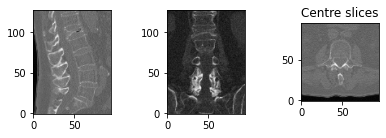
\includegraphics[width=1\linewidth]{images/results_2/original.png}
   \caption{Original image}
   \label{fig:Ng1} 
\end{subfigure}

\begin{subfigure}[b]{0.7\textwidth}
   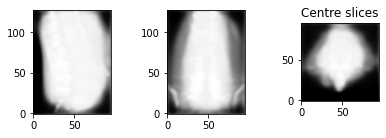
\includegraphics[width=1\linewidth]{images/results_2/binary_mask.png}
   \caption{Predictions of Model 1}
   \label{fig:Ng2}
\end{subfigure}

\begin{subfigure}[b]{0.7\textwidth}
   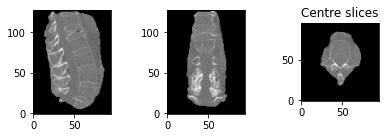
\includegraphics[width=1\linewidth]{images/results_2/binary_segmented.png}
   \caption{Segmented image with Model 1}
   \label{fig:Ng3}
\end{subfigure}

\begin{subfigure}[b]{0.7\textwidth}
   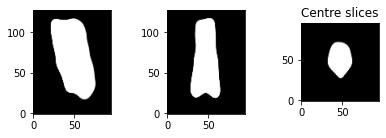
\includegraphics[width=1\linewidth]{images/results_2/dice_mask.png}
   \caption{Predictions of Model 2}
   \label{fig:Ng4}
\end{subfigure}

\begin{subfigure}[b]{0.7\textwidth}
   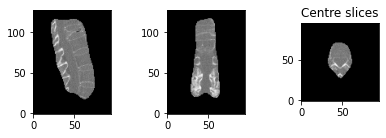
\includegraphics[width=1\linewidth]{images/results_2/dice_segmented.png}
   \caption{Segmented image with Model 2}
   \label{fig:Ng5}
\end{subfigure}

\caption[Results of spine segmentation]{Original and segmented CT image of a spine using Model 1 and Model 2.}
\label{fig:spine-segmentations-1}
\end{figure}

%--------------------------------------------------------------

\begin{figure}[ht!]
\centering
\begin{subfigure}[b]{0.7\textwidth}
   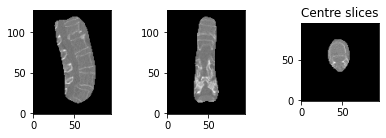
\includegraphics[width=1\linewidth]{images/results_4/1.png}
   \label{fig:Ng1} 
\end{subfigure}

\begin{subfigure}[b]{0.7\textwidth}
   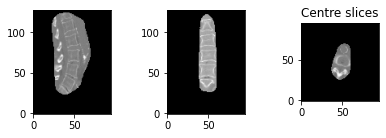
\includegraphics[width=1\linewidth]{images/results_4/2.png}
   \label{fig:Ng2}
\end{subfigure}

\begin{subfigure}[b]{0.7\textwidth}
   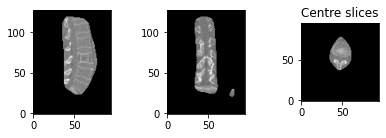
\includegraphics[width=1\linewidth]{images/results_4/3.png}
   \label{fig:Ng3}
\end{subfigure}

\begin{subfigure}[b]{0.7\textwidth}
   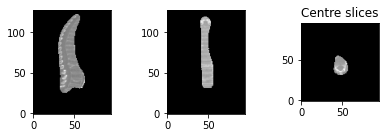
\includegraphics[width=1\linewidth]{images/results_4/4.png}
   \label{fig:Ng4}
\end{subfigure}


\caption[Results of spine segmentation with Model 2]{Segmented images with Model 2}
\label{fig:spine-segmentations-2}
\end{figure}


\chapter{Acronyms}


% \printglossaries
\begin{description}
    \item[AI] Artificial Intelligence
	\item[CNN] Convolutional Neural Network
	\item[CT] Computed Tomography
	\item[ML] Machine Learning
\end{description}


\chapter{Contents of enclosed SD card}

%change appropriately

\begin{figure}
	\dirtree{%
		.1 README.md\DTcomment{the file with SD card contents description}.
		.1 src\DTcomment{the directory of source codes}.
		.2 segmentation\DTcomment{implementation sources}.
		.2 thesis\DTcomment{the directory of \LaTeX{} source codes of the thesis}.
		.1 text\DTcomment{the thesis text directory}.
		.2 thesis.pdf\DTcomment{the thesis text in PDF format}.
	}
\end{figure}

\end{document}
